\documentclass[10pt,a4paper]{article}
\usepackage[T1]{fontenc}
\usepackage[utf8]{inputenc}
\usepackage{lmodern}
\usepackage{microtype}
\usepackage{amsmath,amssymb,mathtools}
\usepackage{graphicx}
\usepackage{geometry}
\usepackage{enumitem}
\geometry{a4paper,margin=20mm,headheight=12pt,footskip=14mm}
\graphicspath{{D014_assets/}}
\setlength{\parindent}{1.2em}
\setlength{\parskip}{0.10em}
\setlength{\emergencystretch}{3em}
\allowdisplaybreaks[2]
\pagestyle{plain}
\begin{document}

% BEGIN ACCEPTED RECORD P0001 / PRINTED 273
% source_sha256=1905043232E1DADD97696372252BB5F91C202EA1B72379E77A9FECBFE9EED4BC
% ndjson_line_sha256=7ee536657f0869ac63e1d3fdd3a98e8f092f0eaab4355e4706490dd6a1e6612f
\begin{center}\LARGE\bfseries Buildings of Generalized Braid Groups\end{center}

\begin{center}\large Pierre Deligne (Bures-sur-Yvette)\end{center}

\section*{Introduction}

The main result of this work is the following.\par

\paragraph{Theorem.} Let \ensuremath{V} be a finite-dimensional real vector space, let \ensuremath{\mathcal{M}} be a finite set of homogeneous hyperplanes of \ensuremath{V,} let \ensuremath{V_C} be the complexification of \ensuremath{V,} and let

\[
Y = V_C - \bigcup_{M\in{}\mathcal{M}} M_C
\]

Assume that the connected components of \ensuremath{V} \ensuremath{-} \ensuremath{\bigcup_{M\in{}\mathcal{M}}} \ensuremath{M} are open simplicial cones. Then \ensuremath{Y} is a \ensuremath{K(\pi{},} 1).\par

Let \ensuremath{V} be as above, and let \ensuremath{W} \ensuremath{\subset{}} \ensuremath{\operatorname{GL}(V)} be a finite group generated by reflections. Suppose that no nonzero vector of \ensuremath{V} is fixed by \ensuremath{W:}\par

\[
V^W = 0
\]

Let \ensuremath{\Phi{}} be any Euclidean structure on \ensuremath{V} invariant under \ensuremath{W,} and let \ensuremath{\mathcal{M}} be the set of hyperplanes \ensuremath{M} such that the orthogonal reflection with respect to \ensuremath{M} belongs to \ensuremath{W.} It is then known that \ensuremath{(V,} \ensuremath{\mathcal{M})} satisfies the hypothesis of the theorem, and that \ensuremath{W} acts freely on the corresponding space \ensuremath{Y_W.} The quotient \ensuremath{X_W} \ensuremath{=} \ensuremath{Y_W/W} is therefore also a \ensuremath{K(\pi{},} 1).\par

This result had been conjectured by Brieskorn. It is new only for \ensuremath{W} of type \ensuremath{H_3,} \ensuremath{H_4,} \ensuremath{E_6,} \ensuremath{E_7,} or \ensuremath{E_8} (Brieskorn [2]). We also give a new proof that the fundamental group of \ensuremath{X_W} is the generalized braid group \ensuremath{\widetilde{W}} corresponding to \ensuremath{W} (Brieskorn [3]).\par

Reduced to the particular case considered above, the plan of the proof is as follows.\par

\hangindent=1.5em\noindent a) We construct a building \ensuremath{I(\widetilde{W})} on which \ensuremath{\widetilde{W}} acts, and a set \ensuremath{\mathcal{S}} of spheres in \ensuremath{I(\widetilde{W}),} isomorphic to the unit sphere of \ensuremath{V.} The group \ensuremath{\widetilde{W}} acts strictly simply transitively on \ensuremath{\mathcal{S}.}\par

\hangindent=1.5em\noindent b) We show that, up to homotopy, \ensuremath{I(\widetilde{W})} is the wedge of the spheres \ensuremath{S\in{}\mathcal{S}.}\par

\hangindent=1.5em\noindent c) We relate \ensuremath{X_W} and \ensuremath{I(\widetilde{W}).}\par

The description of \ensuremath{\mathcal{S}} and the possibility of c) had emerged during a conversation with Brieskorn and Tits in the spring of 1970. The ideas required to establish b) were supplied to me by Garside [4], whom I follow very closely in many places.\par

% END ACCEPTED RECORD P0001

% BEGIN ACCEPTED RECORD P0002 / PRINTED 274
% source_sha256=1905043232E1DADD97696372252BB5F91C202EA1B72379E77A9FECBFE9EED4BC
% ndjson_line_sha256=a75bb318a68a155ecdbfa66dce9b485609a79120e3b9e0ede7c7730d17440595
In Section 4, we determine the center of \ensuremath{\widetilde{W}} and solve the word problem and the conjugacy problem in \ensuremath{\widetilde{W}.} These results were obtained independently by \ensuremath{E.} Brieskorn and \ensuremath{K.} Saito, who, like us, use Garside's methods [4].\par

The geometric language used and the techniques of proof are essentially due to Tits; I was able to familiarize myself with his ideas by attending one of his seminars and through conversations.\par

I am pleased to express my gratitude to him here.\par

\section*{0. Notation}

\paragraph{(0.1)} \ensuremath{L^{+}(D):} the free monoid with identity generated by a set \ensuremath{D.}

\paragraph{(0.2)} L(D): the free group generated by a set \ensuremath{D.}

\paragraph{(0.3)} \ensuremath{A^{-}:} the closure of a subset A of a topological space.

\paragraph{(0.4)} For $x,y$ in a monoid with identity and $n\geq 0$, set
\[\operatorname{prod}(n;x,y)=xyxy\ldots\quad(n\text{ factors});\]
one has $\operatorname{prod}(2n;x,y)=(xy)^n$,
$\operatorname{prod}(2n+1;x,y)=(xy)^n x$.

\section*{1. Galleries}

\paragraph{(1.1)} Let \ensuremath{\mathcal{M}} be a finite set of hyperplanes (the walls) in a finite-dimensional real vector space \ensuremath{V.} We shall use the terminology (walls, chambers, faces, facets) of [1] \ensuremath{V} \S{} 1 (the facets form a partition of \ensuremath{V).} The support \ensuremath{P} of a facet \ensuremath{F} is the intersection of the walls containing \ensuremath{F;} \ensuremath{F} is open in \ensuremath{P.} For every chamber A and every wall \ensuremath{M,} let \ensuremath{D_M(A)} denote the set of chambers on the same side of \ensuremath{M} as A. If A and \ensuremath{B} are two chambers, let \ensuremath{D(A,} \ensuremath{B)} denote the intersection of the \ensuremath{D_M(A)} for which A and \ensuremath{B} are on the same side of \ensuremath{M.} Departing from the terminology of [1] IV 1 ex 15, we shall say that two chambers A and \ensuremath{B} are adjacent if A \ensuremath{\ne{}} \ensuremath{B} and A and \ensuremath{B} have a face in common. We shall use the following elementary facts throughout.

\paragraph{(1.2) Lemma.} (i) Let \ensuremath{M} be a wall of a chamber \ensuremath{B.} There exists a unique chamber \ensuremath{B'} adjacent to \ensuremath{B} and having \ensuremath{M} as a wall. \ensuremath{M} is the only wall separating \ensuremath{B} from \ensuremath{B'.}

\hangindent=1.5em\noindent (ii) Let \ensuremath{B_1,} \ensuremath{B_2,} \ensuremath{B_3} be three chambers, and let \ensuremath{\mathcal{M}(B_i,} \ensuremath{B_j)} be the set of walls separating \ensuremath{B_i} from \ensuremath{B_j.} Then\par

\[
\mathcal{M}(B_1, B_3) = (\mathcal{M}(B_1, B_2) - \mathcal{M}(B_2, B_3)) \cup{} (\mathcal{M}(B_2, B_3) - \mathcal{M}(B_1, B_2))
\]

A gallery of length \ensuremath{n} \ensuremath{(n} \ensuremath{\ge{}} 0), with source A and target \ensuremath{B,} is a sequence of chambers \ensuremath{(C_0,} \ldots{}, \ensuremath{C_n)} with A \ensuremath{=} \ensuremath{C_0,} \ensuremath{C_{i+1}} adjacent to \ensuremath{C_i} (0 \ensuremath{\le{}} i \ensuremath{\le{}} \ensuremath{n),} and \ensuremath{C_n} \ensuremath{=} \ensuremath{B.} The composite of two galleries \ensuremath{G} \ensuremath{=} \ensuremath{(C_0,} \ldots{}, \ensuremath{C_n)} and \ensuremath{G'} \ensuremath{=} \ensuremath{(C'_0,} \ldots{}, \ensuremath{C'_m)}\par

% END ACCEPTED RECORD P0002

% BEGIN ACCEPTED RECORD P0003 / PRINTED 275
% source_sha256=1905043232E1DADD97696372252BB5F91C202EA1B72379E77A9FECBFE9EED4BC
% ndjson_line_sha256=1e7f5b10865dddbf79d11b44206e6e912cdaa7ae826f264f923f5f1f67047970
is defined if \ensuremath{C_n} \ensuremath{=} \ensuremath{C'_0,} and is then\par

\ensuremath{GG'} \ensuremath{=} \ensuremath{(C_0,} \ldots{}, \ensuremath{C_n,} \ensuremath{C'_1,} \ldots{}, \ensuremath{C'_m).}\par

If \ensuremath{G} is a gallery with source A, A.G denotes its target.\par

The opposite gallery G* of a gallery \ensuremath{G} \ensuremath{=} \ensuremath{(C_0,} \ldots{}, \ensuremath{C_n)} is the gallery \ensuremath{(C_n,} \ldots{}, \ensuremath{C_0).} One has \ensuremath{(GG')^{*}} \ensuremath{=} \ensuremath{G'^{*}} G*.\par

The antipodal gallery \ensuremath{-G} of a gallery \ensuremath{G} \ensuremath{=} \ensuremath{(C_0,} \ldots{}, \ensuremath{C_n)} is the sequence of antipodal chambers \ensuremath{-G} \ensuremath{=} \ensuremath{(-C_0,} \ldots{}, \ensuremath{-C_n).}\par

One has \ensuremath{-(GG')} \ensuremath{=} \ensuremath{(-G)(-G'),} and \ensuremath{-(G^{*})} \ensuremath{=} \ensuremath{(-G)^{*}.}\par

The distance d(A, \ensuremath{B)} from a chamber A to a chamber \ensuremath{B} is the least length of a gallery from A to \ensuremath{B.} A gallery from A to \ensuremath{B} is minimal if it has length d(A, \ensuremath{B).}\par

\paragraph{(1.3) Proposition.} The distance d(A, \ensuremath{B)} is the number of walls separating A from \ensuremath{B.} For a gallery \ensuremath{G} from A to \ensuremath{B} to be minimal, it is necessary and sufficient that it cross once the walls separating A from \ensuremath{B} and zero times the others.

It is clear that every gallery from A to \ensuremath{B} crosses every wall separating A from \ensuremath{B,} and it is enough to prove the existence of a gallery \ensuremath{G} from A to \ensuremath{B} whose length equals the number \ensuremath{k} of walls separating A from \ensuremath{B.} We proceed by induction on \ensuremath{k.} The intersection of the \ensuremath{D_M(A),} for \ensuremath{M} a wall of A, is reduced to A. Thus either A \ensuremath{=} \ensuremath{B,} in which case we take \ensuremath{G} \ensuremath{=} (A), or there is a wall \ensuremath{M} of A separating A from \ensuremath{B.} Let \ensuremath{A'} be the chamber adjacent to A having \ensuremath{M} as a wall. \ensuremath{M} is the only wall separating A from \ensuremath{A',} so a wall \ensuremath{N} separates \ensuremath{A'} from \ensuremath{B} if and only if \ensuremath{M} \ensuremath{\ne{}} \ensuremath{N} and \ensuremath{N} separates A from \ensuremath{B.} By the induction hypothesis, there is a gallery \ensuremath{G'} of length \ensuremath{k} \ensuremath{-} 1 from \ensuremath{A'} to \ensuremath{B,} and we take \ensuremath{G} \ensuremath{=} \ensuremath{(AA')G'.}\par

\paragraph{(1.4) Corollary.} Let A, \ensuremath{B,} \ensuremath{C} be three chambers. The following conditions are equivalent.

\hangindent=1.5em\noindent (i) d(A, \ensuremath{C)} \ensuremath{=} d(A, \ensuremath{B)} + d(B, \ensuremath{C),} i.e. there exists a minimal gallery from A to \ensuremath{C} passing through \ensuremath{B.}\par

\hangindent=1.5em\noindent (ii) For a wall to separate A from \ensuremath{C,} it is necessary and sufficient that it separate A from \ensuremath{B} or \ensuremath{B} from \ensuremath{C.} In other words, \ensuremath{\mathcal{M}(A,} \ensuremath{B)} \ensuremath{\subset{}} \ensuremath{\mathcal{M}(A,} \ensuremath{C)} (cf. 1.2(ii)).\par

\hangindent=1.5em\noindent (iii) \ensuremath{B\in{}D(A,} \ensuremath{C).}\par

\paragraph{(1.5) Proposition.} Let \ensuremath{P} be an intersection of walls, let \ensuremath{V_P} \ensuremath{=} V/P, let \ensuremath{pr_P} : \ensuremath{V} \ensuremath{\longrightarrow{}} \ensuremath{V_P} be the projection, and let \ensuremath{\mathcal{M}_P} be the set of hyperplanes \ensuremath{N} of \ensuremath{V_P} such that \ensuremath{pr_P^{-1}(N)} is a wall. Denote by \ensuremath{\pi{}'_P} the unique map from the facets of \ensuremath{(V,} \ensuremath{\mathcal{M})} to those of \ensuremath{(V_P,} \ensuremath{\mathcal{M}_P)} such that \ensuremath{pr_P(F)} \ensuremath{\subset{}} \ensuremath{\pi{}'_P(F).}

\hangindent=1.5em\noindent (i) \ensuremath{\pi{}'_P} respects the incidence relation \ensuremath{F_1} \ensuremath{\subset{}} \ensuremath{F_2^{-}:} if \ensuremath{F_1} \ensuremath{\subset{}} \ensuremath{F_2^{-},} then\par

\ensuremath{\operatorname{codim}(F_1} in \ensuremath{F_2^{-})} \ensuremath{\ge{}} \ensuremath{\operatorname{codim}(\pi{}'_P[F_1]} in \ensuremath{\pi{}'_P[F_2]).}\par

% END ACCEPTED RECORD P0003

% BEGIN ACCEPTED RECORD P0004 / PRINTED 276
% source_sha256=1905043232E1DADD97696372252BB5F91C202EA1B72379E77A9FECBFE9EED4BC
% ndjson_line_sha256=413761eb165043b0557871c64edfe0613bc1d05815db72a1d0292ff18e05ccc9
\ensuremath{\pi{}'_P} takes chambers to chambers; if A and \ensuremath{B} are adjacent, either \ensuremath{\pi{}'_P(A)} \ensuremath{=} \ensuremath{\pi{}'_P(B),} or \ensuremath{\pi{}'_P(A)} and \ensuremath{\pi{}'_P(B)} are adjacent.\par

\hangindent=1.5em\noindent (ii) Let \ensuremath{F} be a facet with support \ensuremath{P} (1.1). The restriction of \ensuremath{\pi{}'_P} to the set of facets \ensuremath{E} of \ensuremath{(V,} \ensuremath{\mathcal{M})} such that \ensuremath{F} \ensuremath{\subset{}} \ensuremath{E^{-}} is bijective. Like its inverse \ensuremath{\pi{}_F,} it preserves codimension, the incidence \ensuremath{E_1} \ensuremath{\subset{}} \ensuremath{E_2^{-},} and hence adjacency of chambers. We shall also write \ensuremath{\pi{}_F} for the bijection \ensuremath{pr_P^{-1}} between intersections of walls in \ensuremath{V_P} and intersections of walls in \ensuremath{V} containing \ensuremath{P.}\par

\hangindent=1.5em\noindent (iii) If \ensuremath{C} \ensuremath{=} \ensuremath{\pi{}_F(C'),} then, for every chamber \ensuremath{X} of \ensuremath{(V,} \ensuremath{\mathcal{M}),}\par

\ensuremath{\pi{}_F^{-1}D(C,} \ensuremath{X)} \ensuremath{=} \ensuremath{D(C',} \ensuremath{\pi{}'_P(X))} and \ensuremath{\pi{}_F^{-1}\mathcal{M}(C,} \ensuremath{X)} \ensuremath{=} \ensuremath{\mathcal{M}_P(C',} \ensuremath{\pi{}'_P(X)).}\par

For \ensuremath{X} \ensuremath{=} \ensuremath{\pi{}_F(X'),} one has\par

\ensuremath{\pi{}_F(D(C',} \ensuremath{X'))} \ensuremath{=} \ensuremath{D(C,} \ensuremath{X)} and \ensuremath{\pi{}_F(\mathcal{M}_P(C',} \ensuremath{X'))} \ensuremath{=} \ensuremath{\mathcal{M}(C,} \ensuremath{X);}\par

\ensuremath{\pi{}_F} then induces a bijection between minimal galleries from \ensuremath{C'} to \ensuremath{X'} and from \ensuremath{C} to \ensuremath{X.}\par

The verification is left to the reader ((iii) follows from 1.4(ii) \ensuremath{\Longleftrightarrow} (iii)).\par

\paragraph{(1.6) Notation.} (i) For \ensuremath{F} a facet with support \ensuremath{P,} \ensuremath{V_P,} \ensuremath{\mathcal{M}_P,} \ensuremath{pr_P,} \ensuremath{\pi{}'_P} are also denoted \ensuremath{V_F,} \ensuremath{\mathcal{M}_F,} \ensuremath{pr_F,} \ensuremath{\pi{}'_F.}

\hangindent=1.5em\noindent (ii) Let \ensuremath{P} be an intersection of walls and \ensuremath{C} a chamber. Suppose that there is a facet of \ensuremath{C} (i.e. in \ensuremath{C^{-})} with support \ensuremath{P.} This facet is then unique. Denote it by F(P), and set\par

\[
C.\Delta{}(P) = \pi{}_{F(P)}(-\pi{}_{F(P)}^{-1}(C))
\]

\paragraph{(1.7) Lemma.} (i) A wall separates \ensuremath{C} from \ensuremath{C.\Delta{}(P)} if and only if it contains \ensuremath{P} ((1.5)(iii)).

\hangindent=1.5em\noindent (ii) If \ensuremath{M} is a wall of \ensuremath{C,} then \ensuremath{C.\Delta{}(M)} is the unique chamber adjacent to \ensuremath{C} and having \ensuremath{M} as a wall (cf. 1.5(iii), 1.2(i)).\par

\hangindent=1.5em\noindent (iii) Let \ensuremath{M} \ensuremath{\ne{}} \ensuremath{N} be two walls of \ensuremath{C} whose intersection \ensuremath{P} contains a facet of \ensuremath{C} open in \ensuremath{P.} There are exactly two minimal galleries from \ensuremath{C} to \ensuremath{C.\Delta{}(P).} One begins with \ensuremath{(C,} \ensuremath{C.\Delta{}(M));} the other begins with \ensuremath{(C,} \ensuremath{C.\Delta{}(N)).}\par

Assertion (iii) is verified by reduction to rank two (cf. 1.5(iii)), where the drawing is\par

(1.7.1)\par

\begin{figure}[htbp]
\centering
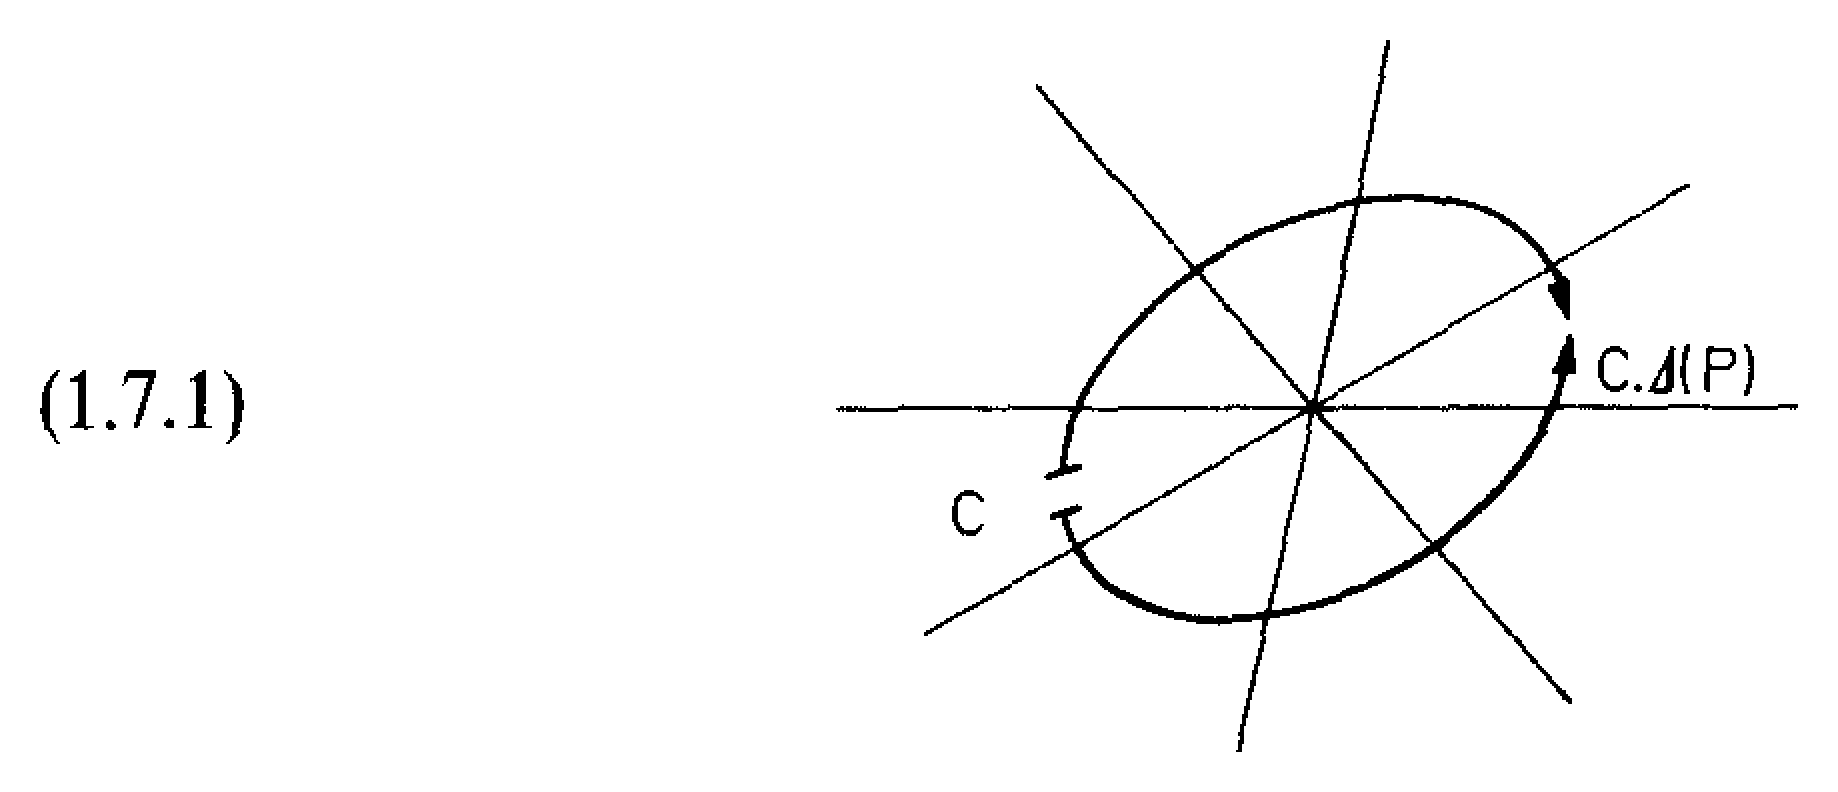
\includegraphics[width=0.78\linewidth]{P0004-A01.png}
\label{fig:p0004-a01}
\end{figure}

% END ACCEPTED RECORD P0004

% BEGIN ACCEPTED RECORD P0005 / PRINTED 277
% source_sha256=1905043232E1DADD97696372252BB5F91C202EA1B72379E77A9FECBFE9EED4BC
% ndjson_line_sha256=9da7b52e491a01c5e6fda53c35e61d3c9171d57f0d90371a3b9e622c5eb1b22c
From now on we assume the following condition.\par

\paragraph{(1.8) Hypothesis.} The chambers are open simplicial cones.

In other words, each chamber is the set of points with coordinates \ensuremath{>} 0 in a suitable basis of \ensuremath{V.}\par

\paragraph{(1.9.1) Remark.} Let \ensuremath{P} be an intersection of walls.

\hangindent=1.5em\noindent (i) \ensuremath{(V_P,} \ensuremath{\mathcal{M}_P)} still satisfies (1.8);\par

\hangindent=1.5em\noindent (ii) the set \ensuremath{\mathcal{M}^P} of traces on \ensuremath{P} of the walls not containing \ensuremath{P} still satisfies (1.8).\par

If \ensuremath{\mathcal{M}} is defined by a ``Weyl group'' \ensuremath{W} (see the introduction), \ensuremath{\mathcal{M}^P} is in general no longer of this type.\par

\paragraph{(1.9.2) Remark.} Hypothesis (1.8) ensures that if \ensuremath{P} is an intersection of walls of a chamber \ensuremath{C,} the condition of (1.6) is satisfied. The chamber \ensuremath{C.\Delta{}(P)} is therefore defined.

\paragraph{(1.10) Definition.} Two galleries \ensuremath{G} and \ensuremath{G'} with the same endpoints are equivalent (notation: \ensuremath{G} \ensuremath{\sim{}} \ensuremath{G')} if there exists a sequence of galleries \ensuremath{G} \ensuremath{=} \ensuremath{G_0,} \ldots{}, \ensuremath{G_n} \ensuremath{=} \ensuremath{G'} \ensuremath{(n} \ensuremath{\ge{}} 0) such that \ensuremath{G_{j+1}} is obtained from \ensuremath{G_j} in the following way (0 \ensuremath{\le{}} j \ensuremath{<} \ensuremath{n):}

\hangindent=1.5em\noindent a) there are decompositions \ensuremath{G_j} \ensuremath{=} \ensuremath{E_1FE_2,} \ensuremath{G_{j+1}} \ensuremath{=} \ensuremath{E_1F'E_2;}\par

\hangindent=1.5em\noindent b) there is a chamber \ensuremath{C} and two walls \ensuremath{M,} \ensuremath{N} of \ensuremath{C} such that \ensuremath{F} and \ensuremath{F'} are the two minimal galleries from \ensuremath{C} to \ensuremath{C.\Delta{}(M} \ensuremath{\cap{}} \ensuremath{N).}\par

Composition of galleries, the operations \ensuremath{G} \ensuremath{\longrightarrow{}} G* and \ensuremath{G} \ensuremath{\longrightarrow{}} \ensuremath{-G,} the source and target maps, and the ``length'' function are compatible with this equivalence relation and therefore pass to the quotient. We shall generally denote classes of galleries by lowercase letters. We say that a class of galleries \ensuremath{e} begins (respectively ends) with a class of galleries f if there exists \ensuremath{g} such that \ensuremath{e} \ensuremath{=} fg (respectively \ensuremath{e} \ensuremath{=} gf). We verify:\par

\paragraph{(1.11) Proposition.} Equivalent galleries cross each wall the same number of times.

\paragraph{(1.12) Proposition.} Two minimal galleries with the same endpoints are equivalent.

Let \ensuremath{G} \ensuremath{=} \ensuremath{(C_0,} \ldots{}, \ensuremath{C_n)} and \ensuremath{G'} \ensuremath{=} \ensuremath{(C'_0,} \ldots{}, \ensuremath{C'_n),} with endpoints A and \ensuremath{B.} We proceed by induction on the length of the galleries under consideration. The case \ensuremath{n} \ensuremath{=} 0 is trivial, and the induction hypothesis allows us to suppose that \ensuremath{C_1} \ensuremath{\ne{}} \ensuremath{C'_1.} Let \ensuremath{M} and \ensuremath{M'} be the walls separating A \ensuremath{=} \ensuremath{C_0} \ensuremath{=} \ensuremath{C'_0} from \ensuremath{C_1} and \ensuremath{C'_1,} and let \ensuremath{C} \ensuremath{=} \ensuremath{A.\Delta{}(M} \ensuremath{\cap{}} \ensuremath{M').} The walls \ensuremath{M} and \ensuremath{M'} separate A from \ensuremath{B.} By reduction to rank two (1.5)(iii), it follows that every wall separating A from \ensuremath{C} separates A from \ensuremath{B}\par

% END ACCEPTED RECORD P0005

% BEGIN ACCEPTED RECORD P0006 / PRINTED 278
% source_sha256=1905043232E1DADD97696372252BB5F91C202EA1B72379E77A9FECBFE9EED4BC
% ndjson_line_sha256=b0756b6c200423190a53a1bf2057dedefe8900f02c5252602e37e88f9e480ade
\begin{figure}[htbp]
\centering
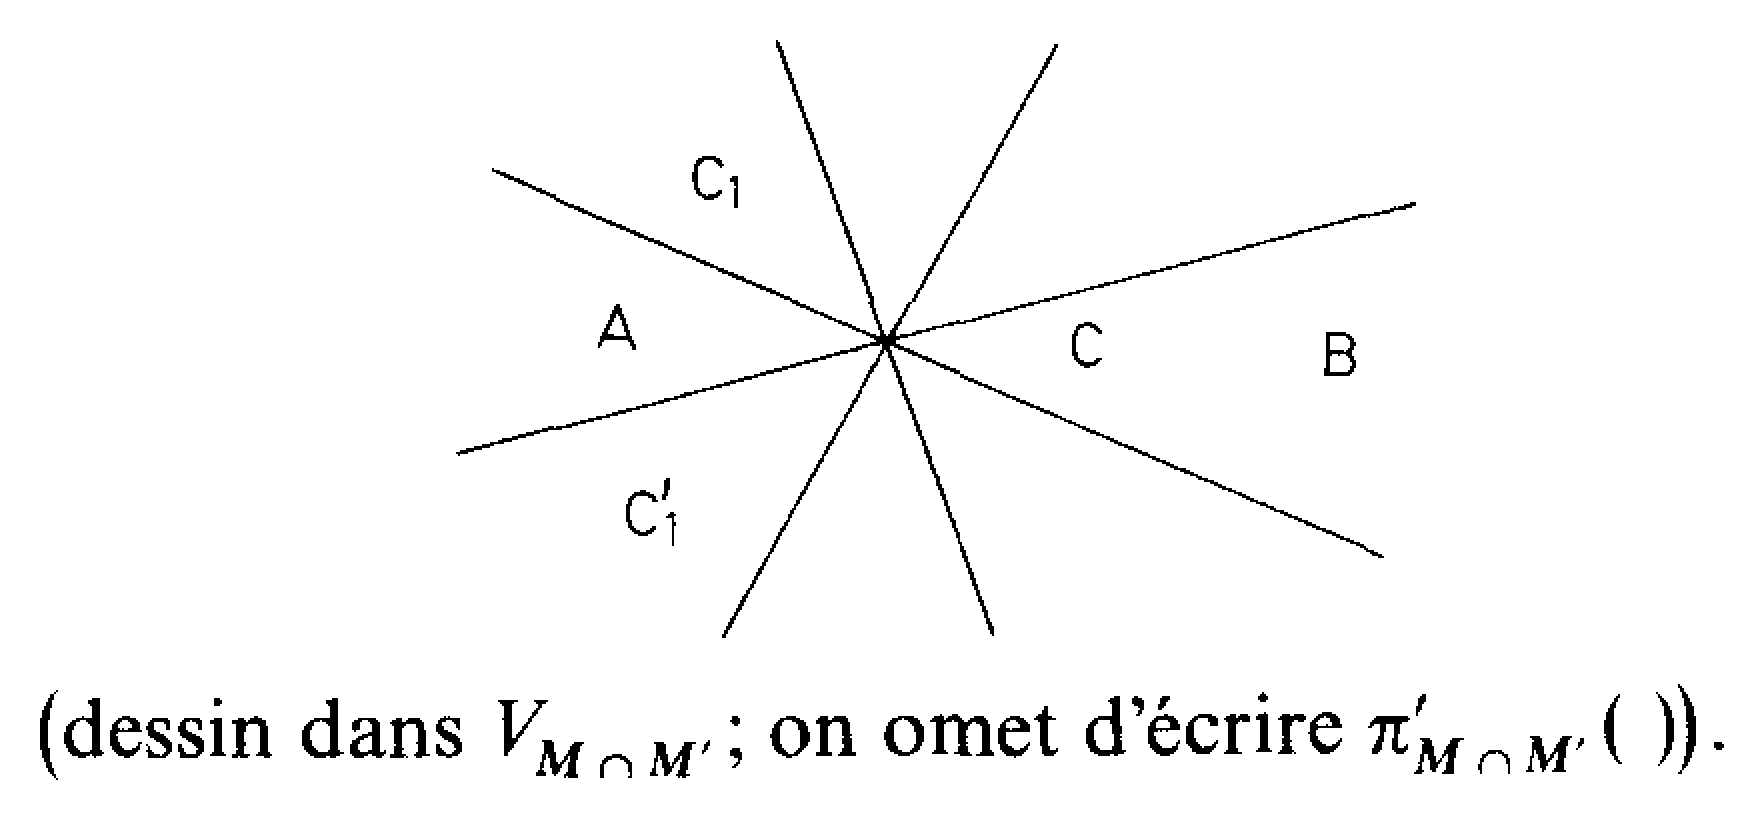
\includegraphics[width=0.78\linewidth]{P0006-A01.png}
\label{fig:p0006-a01}
\end{figure}

(drawing in \ensuremath{V_{M\cap{}M'};} we omit writing \ensuremath{\pi{}'_{M\cap{}M'}(} )).\par

Let \ensuremath{F} (respectively \ensuremath{F')} be the minimal gallery from A to \ensuremath{C} that passes through \ensuremath{C_1} (respectively \ensuremath{C'_1),} and let \ensuremath{E} be a minimal gallery from \ensuremath{C} to \ensuremath{B.} The galleries FE and \ensuremath{F'E} are minimal and equivalent. The minimal galleries \ensuremath{G} and FE (respectively \ensuremath{G'} and \ensuremath{FE')} begin with (A, \ensuremath{C_1)} (respectively with (A, \ensuremath{C'_1)).} The induction hypothesis implies that they are equivalent, and (1.12) follows.\par

\paragraph{(1.13) Notation.} (i) Let \ensuremath{u(A,} \ensuremath{B)} denote the equivalence class of minimal galleries from A to \ensuremath{B.}

\hangindent=1.5em\noindent (ii) For I a set of walls of a chamber \ensuremath{C,} with intersection \ensuremath{P,} set \ensuremath{\Delta{}(P)} \ensuremath{=} \ensuremath{u(C,} \ensuremath{C.\Delta{}(P))} (cf. (1.9.2)). For I the set of all walls, set \ensuremath{\Delta{}} \ensuremath{=} \ensuremath{u(C,} \ensuremath{-C).}\par

The interest of the notation lies in its ambiguity with respect to \ensuremath{C.}\par

\paragraph{(1.14) Proposition.} Let A be a chamber and \ensuremath{\mathcal{G}} a set of classes of galleries of bounded length with source A. Suppose that \ensuremath{\mathcal{G}} satisfies the conjunction (i) of

\hangindent=1.5em\noindent \ensuremath{(i_a)} \ensuremath{(A)\in{}\mathcal{G}.}\par

\hangindent=1.5em\noindent \ensuremath{(i_b)} If \ensuremath{gh\in{}\mathcal{G},} then \ensuremath{g\in{}\mathcal{G}.}\par

\hangindent=1.5em\noindent \ensuremath{(i_c)} Let \ensuremath{g} have target \ensuremath{B,} and let \ensuremath{M,} \ensuremath{N} be two walls of \ensuremath{B.} If \ensuremath{g\Delta{}(M)} and \ensuremath{g\Delta{}(N)} are in \ensuremath{\mathcal{G},} then \ensuremath{g\Delta{}(M} \ensuremath{\cap{}} \ensuremath{N)\in{}\mathcal{G}.}\par

Then\par

\hangindent=1.5em\noindent (ii) There exists a unique class of galleries \ensuremath{x} with source A such that\par

\ensuremath{\mathcal{G}} \ensuremath{=} \{g \ensuremath{|} \ensuremath{x} begins with g\}.\par

Uniqueness is clear: if \ensuremath{x} begins with \ensuremath{y} and \ensuremath{x} \ensuremath{\ne{}} \ensuremath{y,} then \ensuremath{y} has strictly smaller length than \ensuremath{x.} Let \ensuremath{x} have maximal length in \ensuremath{\mathcal{G}.} To ensure that \ensuremath{x} has the required property, it is enough to prove the following assertion.\par

(*) Let \ensuremath{g} and \ensuremath{M} be such that (a) \ensuremath{x} begins with \ensuremath{g} and (b) \ensuremath{x} does not begin with \ensuremath{g\Delta{}(M),} while \ensuremath{g\Delta{}(M)\in{}\mathcal{G}.} Then there exist \ensuremath{g'} and \ensuremath{M'} still satisfying (a) and (b), with \ensuremath{g'} strictly longer than \ensuremath{g.}\par

Since \ensuremath{g\Delta{}(M)\in{}\mathcal{G},} maximality of \ensuremath{x} implies that \ensuremath{g} \ensuremath{\ne{}} \ensuremath{x,} and hence that \ensuremath{x} begins with \ensuremath{g\Delta{}(N)} for a suitable \ensuremath{N,} necessarily distinct from \ensuremath{M.} By \ensuremath{(i_c),} one then has \ensuremath{g\Delta{}(M} \ensuremath{\cap{}} \ensuremath{N)\in{}\mathcal{G}.}\par

% END ACCEPTED RECORD P0006

% BEGIN ACCEPTED RECORD P0007 / PRINTED 279
% source_sha256=1905043232E1DADD97696372252BB5F91C202EA1B72379E77A9FECBFE9EED4BC
% ndjson_line_sha256=76b5ba7a60ffeda764fd9cbf00081055cfb62bd86e33b6b279e0e2ce1b092e81
Since \ensuremath{g\Delta{}(M} \ensuremath{\cap{}} \ensuremath{N)} begins with \ensuremath{g\Delta{}(M),} \ensuremath{x} does not begin with \ensuremath{g\Delta{}(M} \ensuremath{\cap{}} \ensuremath{N).}\par

Let \ensuremath{(C_0,} \ldots{}, \ensuremath{C_m)} be the minimal gallery from A.g to \ensuremath{A.g\Delta{}(M} \ensuremath{\cap{}} \ensuremath{N)} that begins with (A.g, \ensuremath{A.g\Delta{}(N)).} Let i (0 \ensuremath{<} i \ensuremath{<} \ensuremath{m)} be the largest i such that \ensuremath{x} begins with \ensuremath{g'} \ensuremath{=} \ensuremath{g(C_0,} \ldots{}, \ensuremath{C_i).} Then \ensuremath{g'} and the wall \ensuremath{M'} between \ensuremath{C_i} and \ensuremath{C_{i+1}} satisfy (a)(b).\par

\begin{figure}[htbp]
\centering
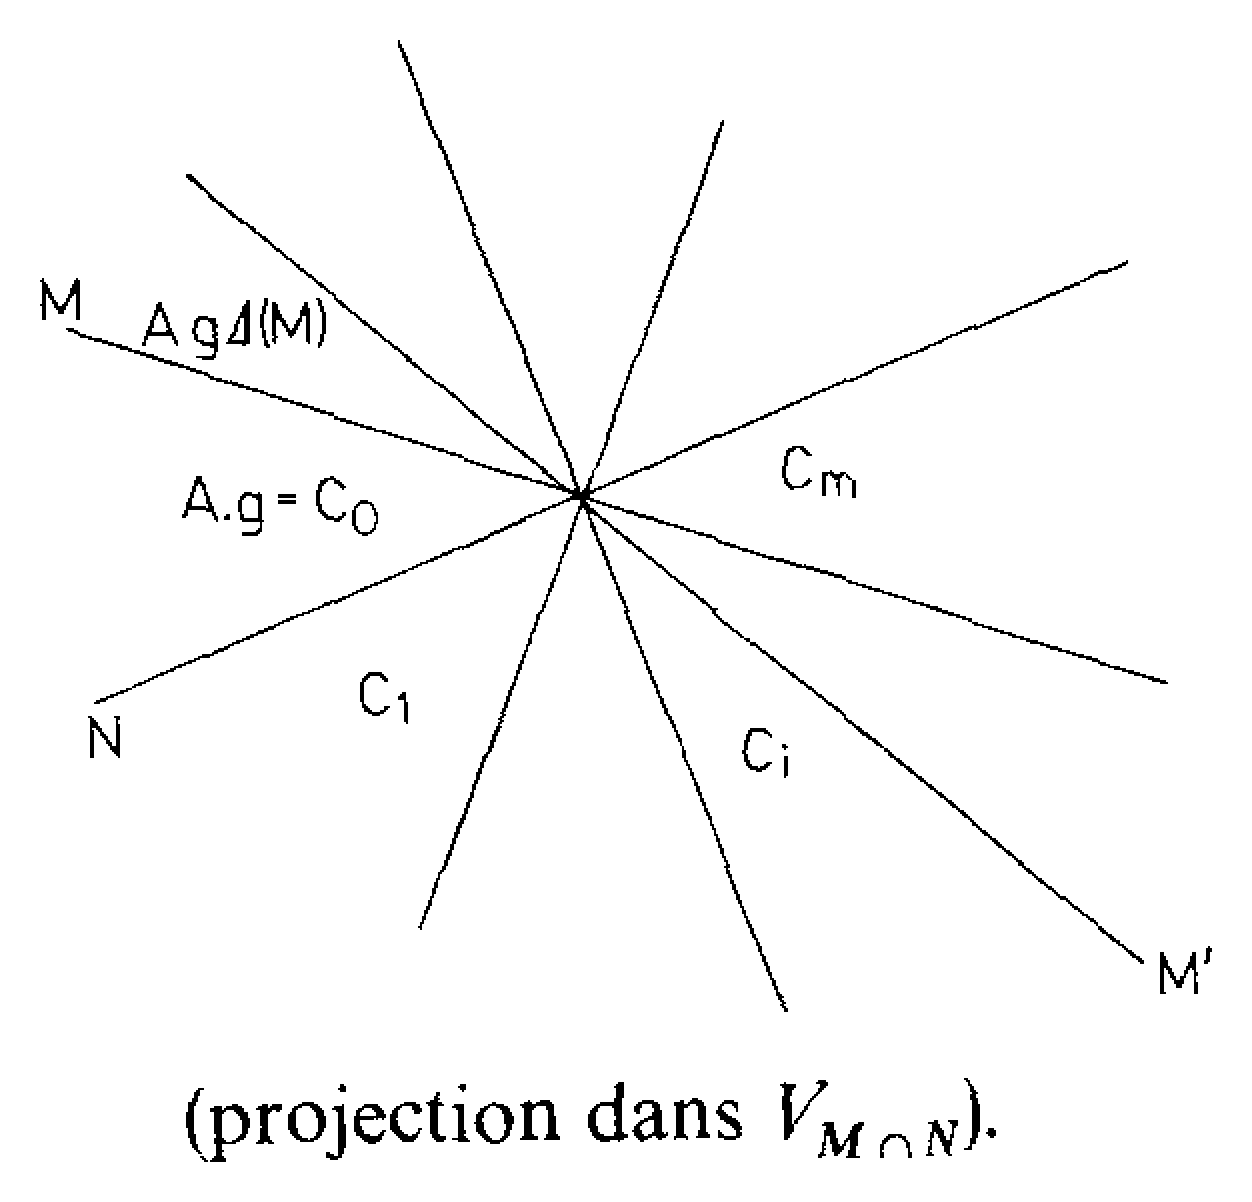
\includegraphics[width=0.56\linewidth]{P0007-A01.png}
\label{fig:p0007-a01}
\end{figure}

(projection in \ensuremath{V_{M\cap{}N}).}\par

\paragraph{(1.15) Proposition.} Let A be a chamber and \ensuremath{\mathcal{B}} a set of chambers. For \ensuremath{\mathcal{B}} to satisfy the conjunction (i) consisting of

\hangindent=1.5em\noindent \ensuremath{(i_a)} \ensuremath{A\in{}\mathcal{B}.}\par

\hangindent=1.5em\noindent \ensuremath{(i_b)} If \ensuremath{B\in{}\mathcal{B},} then \ensuremath{D(A,} \ensuremath{B)\subset{}\mathcal{B}.}\par

\hangindent=1.5em\noindent \ensuremath{(i_c)} Let \ensuremath{M} and \ensuremath{N} be two walls of a chamber \ensuremath{B.} If A and \ensuremath{B} are on the same side of \ensuremath{M} and of \ensuremath{N,} and \ensuremath{B.\Delta{}(M)} and \ensuremath{B.\Delta{}(N)} belong to \ensuremath{\mathcal{B},} then \ensuremath{B.\Delta{}(M} \ensuremath{\cap{}} \ensuremath{N)\in{}\mathcal{B}.}\par

it is necessary and sufficient that\par

\hangindent=1.5em\noindent (ii) There exists a unique chamber \ensuremath{C} such that \ensuremath{\mathcal{B}} \ensuremath{=} \ensuremath{D(A,} \ensuremath{C).}\par

It is easy to verify that (ii) \ensuremath{\Rightarrow} (i). To prove that (i) \ensuremath{\Rightarrow} (ii), apply (1.14) to the set \ensuremath{\mathcal{G}} of the \ensuremath{u(A,} \ensuremath{B)} for \ensuremath{B\in{}\mathcal{B}} (note that, by (1.3) and (1.11), every gallery \ensuremath{G} of class \ensuremath{g} such that some \ensuremath{u(A,} \ensuremath{B)} begins with \ensuremath{g} is automatically minimal), and apply (1.4)(i) \ensuremath{\Longleftrightarrow} (iii) to the gallery class \ensuremath{x} \ensuremath{=} \ensuremath{u(A,} \ensuremath{X)} thereby obtained.\par

Applying criterion (1.15), we find:\par

\paragraph{(1.16) Corollary.} Let A and \ensuremath{B} be two adjacent chambers separated by the wall \ensuremath{M,} and let \ensuremath{C} be on the same side of \ensuremath{M} as \ensuremath{B.} There exists \ensuremath{C'} such that

\[
D(A, C) \cap{} D_M(B) = D(B, C')
\]

\paragraph{(1.17) Corollary.} (i) Let A, \ensuremath{C_1,} \ensuremath{C_2} be three chambers. There exists \ensuremath{C} such that

\paragraph{(1.17.1)} \ensuremath{D(A,} \ensuremath{C)} \ensuremath{=} \ensuremath{D(A,} \ensuremath{C_1)} \ensuremath{\cap{}} \ensuremath{D(A,} \ensuremath{C_2).}

% END ACCEPTED RECORD P0007

% BEGIN ACCEPTED RECORD P0008 / PRINTED 280
% source_sha256=1905043232E1DADD97696372252BB5F91C202EA1B72379E77A9FECBFE9EED4BC
% ndjson_line_sha256=b70f550366b7e21eb711dc46af7bc541fd716731bb1c2c7ff963c6979a6d7741
\hangindent=1.5em\noindent (ii) Let A and \ensuremath{C_1} be two chambers, and let \ensuremath{M} be a wall of A. There exists \ensuremath{C'} such that\par

\paragraph{(1.17.2)} \ensuremath{D(A,} \ensuremath{C')} \ensuremath{=} \ensuremath{D(A,} \ensuremath{C_1)} \ensuremath{\cap{}} \ensuremath{D_M(A).}

In fact, (ii) is the special case of (i) with \ensuremath{C_2} \ensuremath{=} \ensuremath{-(A.\Delta{}(M)).}\par

\paragraph{(1.18) Lemma.} Let \ensuremath{M,} \ensuremath{M',} \ensuremath{M''} be three distinct walls of a chamber A, \ensuremath{A_1} \ensuremath{=} \ensuremath{A.\Delta{}(M),} \ensuremath{B} \ensuremath{=} \ensuremath{A.\Delta{}(M} \ensuremath{\cap{}} \ensuremath{M'} \ensuremath{\cap{}} \ensuremath{M''),} \ensuremath{B'} \ensuremath{=} \ensuremath{A.\Delta{}(M} \ensuremath{\cap{}} \ensuremath{M'),} and \ensuremath{B''} \ensuremath{=} \ensuremath{A.\Delta{}(M} \ensuremath{\cap{}} \ensuremath{M'').} For every chamber \ensuremath{C,} if \ensuremath{B'\in{}D(A_1,} \ensuremath{C)} and \ensuremath{B''\in{}D(A_1,} \ensuremath{C),} then \ensuremath{B\in{}D(A_1,} \ensuremath{C).}

The facet \ensuremath{F} of A open in \ensuremath{M} \ensuremath{\cap{}} \ensuremath{M'} \ensuremath{\cap{}} \ensuremath{M''} is a facet of all the chambers A, \ensuremath{A_1,} \ensuremath{B,} \ensuremath{B',} and \ensuremath{B''.} Applying (1.5)(iii), we may therefore reduce to the case dim \ensuremath{V} \ensuremath{=} 3. Applying (1.17)(ii), we may further suppose that \ensuremath{A_1} and \ensuremath{C} are on the same side of \ensuremath{M.} Make these assumptions, and suppose that \ensuremath{B',} \ensuremath{B''\in{}D(A_1,} \ensuremath{C).} Since \ensuremath{M'} (respectively \ensuremath{M'')} separates \ensuremath{A_1} from \ensuremath{B'} (respectively \ensuremath{B''),} \ensuremath{A_1} and \ensuremath{C} are separated by \ensuremath{M'} and \ensuremath{M''} (and are on the same side of \ensuremath{M);} hence A and \ensuremath{C} are separated by \ensuremath{M,} \ensuremath{M',} and \ensuremath{M'',} and \ensuremath{C} \ensuremath{=} \ensuremath{-A} \ensuremath{=} \ensuremath{B.}\par

The following key result is inspired by [4].\par

\paragraph{(1.19) Proposition.} (i) Let A, \ensuremath{B,} \ensuremath{C} be three chambers, \ensuremath{F} a gallery from A to \ensuremath{B,} and \ensuremath{G_1,} \ensuremath{G_2} two galleries from \ensuremath{B} to \ensuremath{C.} If \ensuremath{FG_1} \ensuremath{\sim{}} \ensuremath{FG_2,} then \ensuremath{G_1} \ensuremath{\sim{}} \ensuremath{G_2.}

\hangindent=1.5em\noindent (ii) Similarly, if \ensuremath{G_1E} \ensuremath{\sim{}} \ensuremath{G_2E,} then \ensuremath{G_1} \ensuremath{\sim{}} \ensuremath{G_2.}\par

\hangindent=1.5em\noindent (iii) Let \ensuremath{g} be an equivalence class of galleries with source A. There exists a chamber \ensuremath{C} such that \ensuremath{g} begins with \ensuremath{u(A,} \ensuremath{B)} if and only if \ensuremath{B\in{}D(A,} \ensuremath{C).}\par

Statement (ii) follows from (i) by passing to opposite galleries.\par

Let \ensuremath{G} \ensuremath{=} \ensuremath{(C_0,} \ldots{}, \ensuremath{C_n)} and \ensuremath{G'} \ensuremath{=} \ensuremath{(C'_0,} \ldots{}, \ensuremath{C'_n)} be two galleries of length \ensuremath{n} with the same endpoints. If \ensuremath{n} \ensuremath{\ge{}} 1, set \ensuremath{G_1} \ensuremath{=} \ensuremath{(C_1,} \ldots{}, \ensuremath{C_n)} and \ensuremath{G'_1} \ensuremath{=} \ensuremath{(C'_1,} \ldots{}, \ensuremath{C'_n).} If moreover \ensuremath{C_1} \ensuremath{\ne{}} \ensuremath{C'_1,} let \ensuremath{M} and \ensuremath{M'} be the walls separating \ensuremath{C_0} \ensuremath{=} \ensuremath{C'_0} from \ensuremath{C_1} and \ensuremath{C'_1,} and set A \ensuremath{=} \ensuremath{C_0.\Delta{}(M} \ensuremath{\cap{}} \ensuremath{M').} Consider the following relation \ensuremath{R_n(G,} \ensuremath{G')} between galleries \ensuremath{G} and \ensuremath{G'} as above.\par

\ensuremath{R_n(G,} \ensuremath{G')} \ensuremath{\Longleftrightarrow} one of the following holds:\par

\hangindent=2.5em\noindent\hspace*{1.5em}$\alpha{})$ \ensuremath{n} \ensuremath{=} 0;\par

\hangindent=2.5em\noindent\hspace*{1.5em}$\beta{})$ \ensuremath{n} \ensuremath{\ne{}} 0, \ensuremath{C_1} \ensuremath{=} \ensuremath{C'_1,} and \ensuremath{G_1} \ensuremath{\sim{}} \ensuremath{G'_1;}\par

\hangindent=2.5em\noindent\hspace*{1.5em}$\gamma{})$ \ensuremath{n} \ensuremath{\ne{}} 0, \ensuremath{C_1} \ensuremath{\ne{}} \ensuremath{C'_1,} and there exists a gallery \ensuremath{F} from A to \ensuremath{C_n} \ensuremath{=} \ensuremath{C'_n} such that \ensuremath{G_1} \ensuremath{\sim{}} \ensuremath{u(C_1,} A).F and \ensuremath{G'_1} \ensuremath{\sim{}} \ensuremath{u(C'_1,} A).F.\par

We shall prove by induction on \ensuremath{n} the following assertion:\par

\ensuremath{(A_n)} \ensuremath{R_n} is an equivalence relation.\par

Assume \ensuremath{(A_i)} for i \ensuremath{<} \ensuremath{n,} and prove (1.19.1) through (1.19.3) below.\par

\paragraph{(1.19.1)} For galleries of length i \ensuremath{<} \ensuremath{n,} \ensuremath{R_i(G,} \ensuremath{G')} \ensuremath{\Longleftrightarrow} \ensuremath{G} \ensuremath{\sim{}} \ensuremath{G'.}

It is trivial that \ensuremath{R_i(G,} \ensuremath{G')} \ensuremath{\Rightarrow} \ensuremath{G} \ensuremath{\sim{}} \ensuremath{G';} and, with the notation of (1.10), if \ensuremath{G} \ensuremath{\sim{}} \ensuremath{G',} then \ensuremath{R_i(G_j,} \ensuremath{G_{j+1}).}\par

\paragraph{(1.19.2)} Assertion (i) is true for \ensuremath{FG_1} of length \ensuremath{<} \ensuremath{n.}

This follows from (1.19.1) and the second clause in the definition of the \ensuremath{R_i.}\par

% END ACCEPTED RECORD P0008

% BEGIN ACCEPTED RECORD P0009 / PRINTED 281
% source_sha256=1905043232E1DADD97696372252BB5F91C202EA1B72379E77A9FECBFE9EED4BC
% ndjson_line_sha256=e12724088e708b923f713645ffb2689911b5eb46f5b4a7284f0ab4471586875a
\paragraph{(1.19.3)} Assertion (iii) is true for \ensuremath{g} of length \ensuremath{<} \ensuremath{n.}

This follows from (1.15) applied to the set \ensuremath{\mathcal{B}} of chambers \ensuremath{B} such that \ensuremath{g} begins with \ensuremath{u(A,} \ensuremath{B):} hypothesis \ensuremath{(i_c)} of (1.15) is verified using (1.19.2), (1.18), and the third clause in the definition of the \ensuremath{R_i.}\par

It remains to prove that if \ensuremath{G,} \ensuremath{G',} and \ensuremath{G''} are three galleries of length \ensuremath{n} from A to \ensuremath{C,} and \ensuremath{R_n(G,} \ensuremath{G')} and \ensuremath{R_n(G,} \ensuremath{G''),} then \ensuremath{R_n(G',} \ensuremath{G'').} If \ensuremath{n} \ensuremath{=} 0, or \ensuremath{C_1} \ensuremath{=} \ensuremath{C'_1,} or \ensuremath{C_1} \ensuremath{=} \ensuremath{C''_1,} this is trivial.\par

For \ensuremath{n} \ensuremath{>} 0, denote by \ensuremath{M,} \ensuremath{M',} \ensuremath{M''} the walls separating A \ensuremath{=} \ensuremath{C_0} \ensuremath{=} \ensuremath{C'_0} \ensuremath{=} \ensuremath{C''_0} from \ensuremath{C_1,} \ensuremath{C'_1,} and \ensuremath{C''_1.} Distinguish two cases.\par

\paragraph{Case 1.} \ensuremath{C_1} \ensuremath{\ne{}} \ensuremath{C'_1} \ensuremath{=} \ensuremath{C''_1.} Let \ensuremath{B} \ensuremath{=} \ensuremath{A.\Delta{}(M} \ensuremath{\cap{}} \ensuremath{M').} By hypothesis,

\ensuremath{(C_1,} \ldots{}, \ensuremath{C_n)} \ensuremath{\sim{}} \ensuremath{u(C_1,} \ensuremath{B)F'} \ensuremath{\sim{}} \ensuremath{u(C_1,} \ensuremath{B)F'',}\par

\ensuremath{(C'_1,} \ldots{}, \ensuremath{C'_n)} \ensuremath{\sim{}} \ensuremath{u(C'_1,} \ensuremath{B)F',}\par

\ensuremath{(C''_1,} \ldots{}, \ensuremath{C''_n)} \ensuremath{\sim{}} \ensuremath{u(C''_1,} \ensuremath{B)F''.}\par

It follows from (1.19.2) that \ensuremath{F'} \ensuremath{\sim{}} \ensuremath{F'',} and hence that \ensuremath{R_n(G',} \ensuremath{G'').}\par

\paragraph{Case 2.} \ensuremath{C_1} \ensuremath{\ne{}} \ensuremath{C'_1} \ensuremath{\ne{}} \ensuremath{C''_1} \ensuremath{\ne{}} \ensuremath{C_1.} Let \ensuremath{B_1} \ensuremath{=} \ensuremath{A.\Delta{}(M'} \ensuremath{\cap{}} \ensuremath{M''),} \ensuremath{B'} \ensuremath{=} \ensuremath{A.\Delta{}(M} \ensuremath{\cap{}} \ensuremath{M'),} \ensuremath{B''} \ensuremath{=} \ensuremath{A.\Delta{}(M} \ensuremath{\cap{}} \ensuremath{M''),} and \ensuremath{B} \ensuremath{=} \ensuremath{A.\Delta{}(M} \ensuremath{\cap{}} \ensuremath{M'} \ensuremath{\cap{}} \ensuremath{M'').} We have

\[
G_1 = (C_1, \ldots{}, C_n) \sim{} u(C_1, B')F' \sim{} u(C_1, B'')F''
\]

\[
G'_1 = (C'_1, \ldots{}, C'_n) \sim{} u(C'_1, B')F'
\]

\[
G''_1 = (C''_1, \ldots{}, C''_n) \sim{} u(C''_1, B'')F''
\]

so that the class \ensuremath{g_1} of \ensuremath{G_1} begins with \ensuremath{u(C_1,} \ensuremath{B')} and \ensuremath{u(C_1,} \ensuremath{B'').} It then follows from (1.19.3) and Lemma (1.18) that \ensuremath{g_1} begins with \ensuremath{u(C_1,} \ensuremath{B):} \ensuremath{G_1} \ensuremath{\sim{}} \ensuremath{u(C_1,} B)F. By (1.19.2), \ensuremath{F'} \ensuremath{\sim{}} \ensuremath{u(B',} B)F and \ensuremath{F''} \ensuremath{\sim{}} \ensuremath{u(B'',} B)F; hence \ensuremath{G_1} \ensuremath{\sim{}} \ensuremath{u(C_1,} B)F, \ensuremath{G'_1} \ensuremath{\sim{}} \ensuremath{u(C'_1,} B)F, and \ensuremath{G''_1} \ensuremath{\sim{}} \ensuremath{u(C''_1,} B)F. Therefore,\par

\ensuremath{G'_1} \ensuremath{\sim{}} \ensuremath{u(C'_1,} \ensuremath{B_1)u(B_1,} B)F\par

\ensuremath{G''_1} \ensuremath{\sim{}} \ensuremath{u(C''_1,} \ensuremath{B_1)u(B_1,} B)F,\par

so that \ensuremath{R_n(G',} \ensuremath{G'').}\par

\begin{figure}[htbp]
\centering
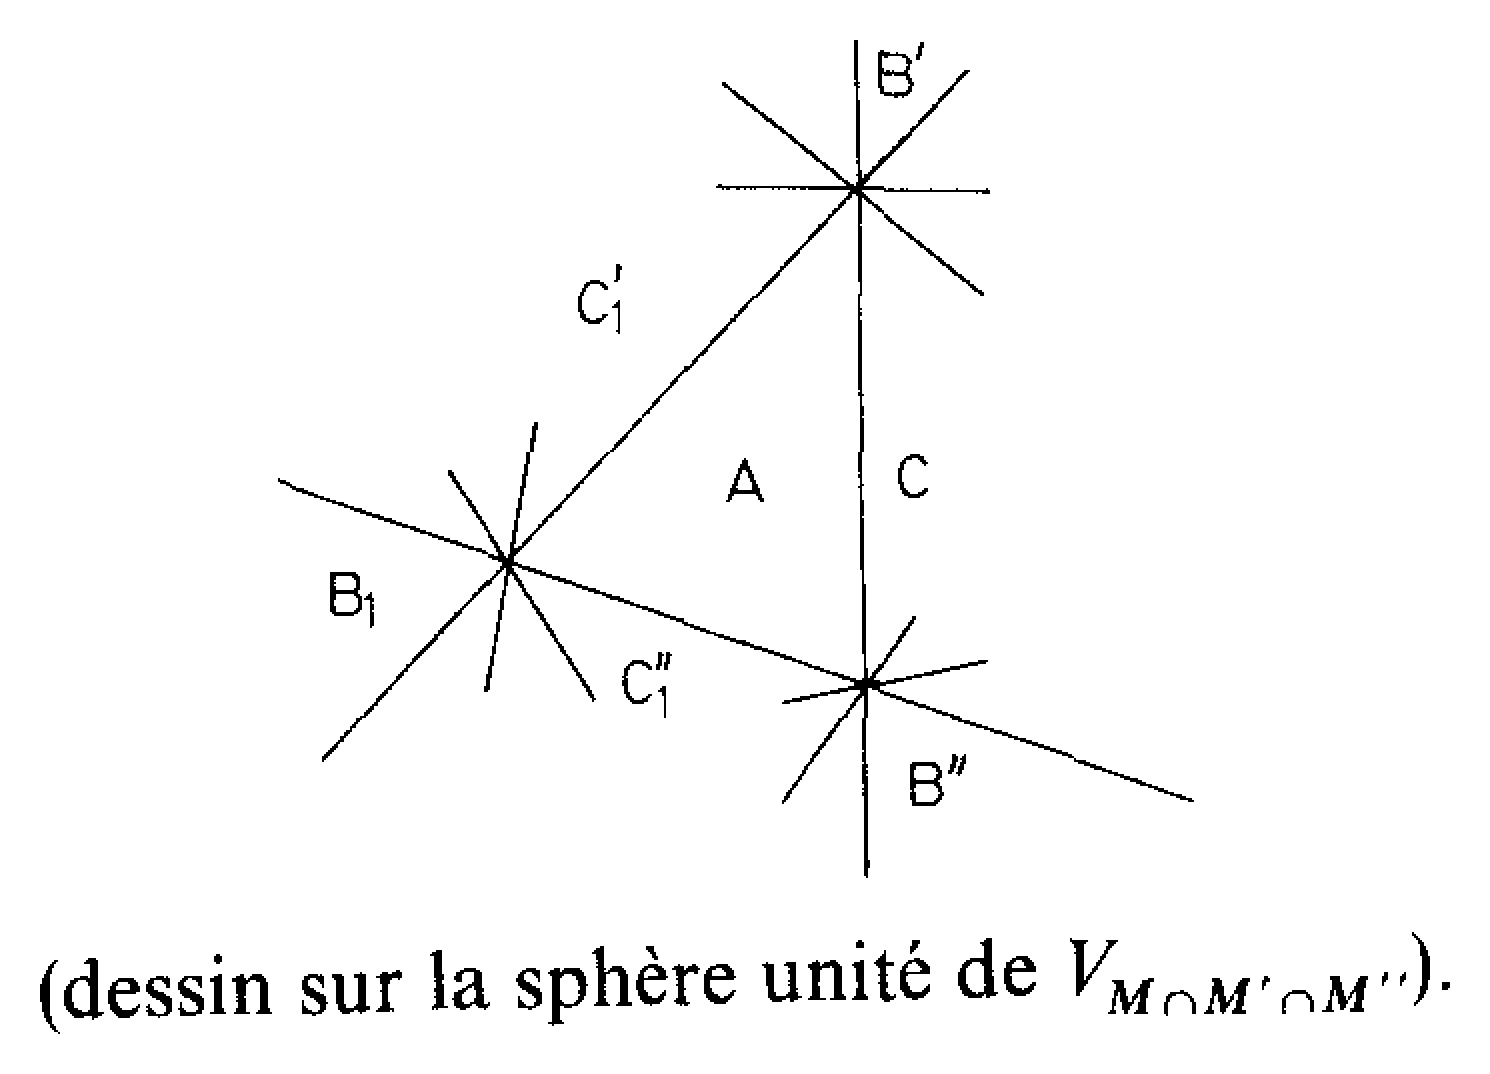
\includegraphics[width=0.62\linewidth]{P0009-A01.png}
\label{fig:p0009-a01}
\end{figure}

(drawing on the unit sphere of \ensuremath{V_{M\cap{}M'\cap{}M''}).}\par

% END ACCEPTED RECORD P0009

% BEGIN ACCEPTED RECORD P0010 / PRINTED 282
% source_sha256=1905043232E1DADD97696372252BB5F91C202EA1B72379E77A9FECBFE9EED4BC
% ndjson_line_sha256=77da59a587ceba4210caec495cece84d5667a7170b4c84ea942c7d31a5685f71
\paragraph{(1.20) Corollary.} Conditions (i) and (ii) of (1.14) are equivalent.

Assume (ii) and prove \ensuremath{(i_c).} Under the hypotheses of \ensuremath{(i_c),} if \ensuremath{x} \ensuremath{=} gh \ensuremath{(h} with source \ensuremath{B),} then (1.19)(i) implies that \ensuremath{h} begins with \ensuremath{\Delta{}(M)} and \ensuremath{\Delta{}(N).} Let \ensuremath{C} be the chamber guaranteed by (1.19)(iii) for \ensuremath{h.} Since \ensuremath{M} and \ensuremath{N} separate \ensuremath{B} from \ensuremath{C,} \ensuremath{\pi{}'_{M\cap{}N}(C)} can only be \ensuremath{\pi{}'_{M\cap{}N}(B).\Delta{},} and \ensuremath{(i_c)} follows from (1.5)(iii).\par

\begin{figure}[htbp]
\centering
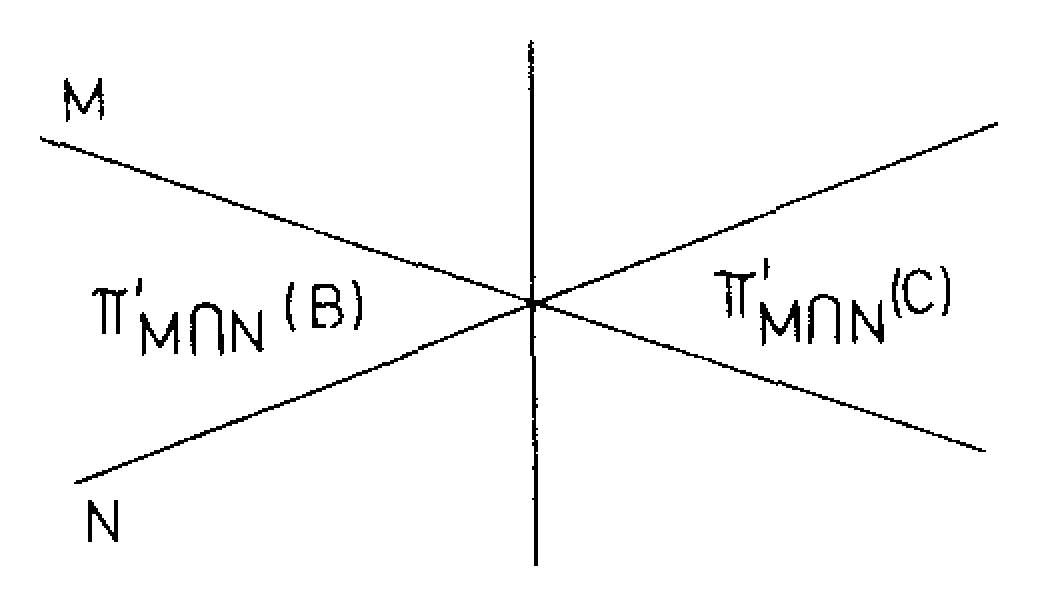
\includegraphics[width=0.54\linewidth]{P0010-A01.png}
\label{fig:p0010-a01}
\end{figure}

\paragraph{(1.21) Corollary.} For every chamber A, let n(A, i) be the number of classes of galleries with source A and length i. Set

\[
f_A = \sum{}_{0}^{\infty{}} n(A, i)t^i \in{} \mathbb{Z}[[t]]
\]

For every chamber A, and for \ensuremath{P} running through the intersections of walls of A (including \{0\} and \ensuremath{V),} one has\par

\[
\sum{}_P (-1)^{\operatorname{codim}(P)} t^{d(A, A.\Delta{}(P))} f_{A.\Delta{}(P)} = 1
\]

This expresses that\par

\hangindent=1.5em\noindent a) the number of classes of galleries of length i that begin with \ensuremath{\Delta{}(P)} is \ensuremath{n(A.\Delta{}(P),} i \ensuremath{-} d(A, \ensuremath{A.\Delta{}(P)))} ((1.19)(i));\par

\hangindent=1.5em\noindent b) classes of galleries that begin with \ensuremath{\Delta{}(P)} and \ensuremath{\Delta{}(Q)} begin with \ensuremath{\Delta{}(P} \ensuremath{\cap{}} \ensuremath{Q)} (by (1.19)(iii)).\par

\paragraph{(1.22) Algorithm.} Let \ensuremath{G} \ensuremath{=} \ensuremath{(A_0,} \ldots{}, \ensuremath{A_n)} be a gallery of length \ensuremath{n} \ensuremath{\ge{}} 1, let \ensuremath{G_1} \ensuremath{=} \ensuremath{(A_1,} \ldots{}, \ensuremath{A_n),} let \ensuremath{M} be the wall separating \ensuremath{A_0} from \ensuremath{A_1,} let \ensuremath{C} be the chamber whose existence is guaranteed by (1.19)(iii) (for \ensuremath{G),} and let \ensuremath{C_1} be the analogous chamber for \ensuremath{G_1.} One can compute \ensuremath{C} recursively using the following formula (cf. (1.16)):

\paragraph{(1.22.1)} \ensuremath{D(A_1,} \ensuremath{C)} \ensuremath{=} \ensuremath{D_M(A_1)} \ensuremath{\cap{}} \ensuremath{D(A_1,} \ensuremath{C_1).}

Since \ensuremath{A_1\in{}D(A,} \ensuremath{C),} \ensuremath{M} indeed separates A from \ensuremath{C} and \ensuremath{C\in{}D_M(A_1).} By (1.19)(i), one also has \ensuremath{D(A_1,} \ensuremath{C)\subset{}D(A_1,} \ensuremath{C_1),} giving the inclusion \ensuremath{\subset{}.} Finally, if \ensuremath{B\in{}D_M(A_1)} \ensuremath{\cap{}} \ensuremath{D(A_1,} \ensuremath{C_1),} then \ensuremath{G_1} begins with \ensuremath{u(A_1,} \ensuremath{B)} and \ensuremath{G} begins with \ensuremath{u(A,} \ensuremath{A_1).u(A_1,} \ensuremath{B)} \ensuremath{=} \ensuremath{u(A,} \ensuremath{B),} which proves (1.22.1).\par

\paragraph{(1.23) Corollary.} Let \ensuremath{G} and \ensuremath{H} be two composable galleries. Let A be the source of \ensuremath{G,} \ensuremath{B} that of \ensuremath{H,} and let \ensuremath{C} be guaranteed by (1.19)(iii): one has \ensuremath{H} \ensuremath{\sim{}} \ensuremath{u(B,} \ensuremath{C).H'.} Then, for every chamber \ensuremath{D,} for the class of GH to begin with \ensuremath{u(A,} \ensuremath{D),} it is necessary (and sufficient) that the class of Gu(B, \ensuremath{C)} begin with \ensuremath{u(A,} \ensuremath{D).}

% END ACCEPTED RECORD P0010

% BEGIN ACCEPTED RECORD P0011 / PRINTED 283
% source_sha256=1905043232E1DADD97696372252BB5F91C202EA1B72379E77A9FECBFE9EED4BC
% ndjson_line_sha256=c4001bbc2c4ffbdeb273ff19553403016980d33248470532cc18d7ee29b0aaad
\paragraph{(1.24) Proposition.} Let A be a chamber, \ensuremath{P} an intersection of walls of A, \ensuremath{F} \ensuremath{=} F(P) (1.6), and \ensuremath{g} an equivalence class of galleries with source A. There exists a class of galleries \ensuremath{g'} of \ensuremath{(V_P,} \ensuremath{\mathcal{M}_P),} with source \ensuremath{\pi{}_F^{-1}(A),} such that, for every gallery \ensuremath{H} of \ensuremath{(V_P,} \ensuremath{\mathcal{M}_P),} \ensuremath{g} begins with \ensuremath{\pi{}_F(H)} if and only if \ensuremath{g'} begins with \ensuremath{H.}

Let \ensuremath{\mathcal{G}} be the set of classes of galleries \ensuremath{h} with source \ensuremath{\pi{}_F^{-1}(A)} in \ensuremath{(V_P,} \ensuremath{\mathcal{M}_P)} such that \ensuremath{g} begins with \ensuremath{\pi{}_F(h).} Apply (1.14) to \ensuremath{(V_P,} \ensuremath{\mathcal{M}_P)} and to \ensuremath{\mathcal{G}.} By (1.19), condition (i) is satisfied (cf. the proof of (1.20)), and (1.24) follows from (1.14)(ii).\par

\paragraph{(1.25)} One may regard the set of galleries as the set of arrows of a category \ensuremath{\operatorname{Gal}_0(V,} \ensuremath{\mathcal{M})} whose objects are the chambers. Similarly, equivalence classes of galleries are the arrows of a quotient category \ensuremath{\operatorname{Gal}_+(V,} \ensuremath{\mathcal{M}).} Let A, \ensuremath{B,} and \ensuremath{C} be three chambers, \ensuremath{E} a gallery from A to \ensuremath{B,} and \ensuremath{F} a gallery from \ensuremath{B} to \ensuremath{C.} Although the general categorical conventions are different, we shall continue to write EF for the composite of \ensuremath{E} and \ensuremath{F.} The operation * (respectively \ensuremath{G} \ensuremath{\longrightarrow{}} \ensuremath{-G)} is an anti-equivalence (respectively an equivalence) of \ensuremath{\operatorname{Gal}_0(V,} \ensuremath{\mathcal{M})} or \ensuremath{\operatorname{Gal}_+(V,} \ensuremath{\mathcal{M})} with itself, inducing the identity (respectively \ensuremath{C} \ensuremath{\longrightarrow{}} \ensuremath{-C)} on the set of objects.

When there is no risk of confusion, we shall write simply \ensuremath{\operatorname{Gal}_0} and \ensuremath{\operatorname{Gal}_+} for \ensuremath{\operatorname{Gal}_0(V,} \ensuremath{\mathcal{M})} and \ensuremath{\operatorname{Gal}_+(V,} \ensuremath{\mathcal{M})} (or for a category \ensuremath{\operatorname{Gal}_0(V_P,} \ensuremath{\mathcal{M}_P)} or \ensuremath{\operatorname{Gal}_+(V_P,} \ensuremath{\mathcal{M}_P)).} By abuse of language, we shall often call the arrows of \ensuremath{\operatorname{Gal}_+} galleries.\par

\paragraph{(1.26) Lemma.} (i) In \ensuremath{\operatorname{Gal}_+,} for every gallery \ensuremath{g,} one has

\[
g\Delta{} = \Delta{}(-g)
\]

\hangindent=1.5em\noindent (ii) For any \ensuremath{g} and \ensuremath{h} with source A in \ensuremath{\operatorname{Gal}_+,} there exists \ensuremath{n} such that \ensuremath{g\Delta{}^n} begins with \ensuremath{h.} If \ensuremath{h} is composed of \ensuremath{k} galleries \ensuremath{u(A_i,} \ensuremath{A_{i+1}),} one may take \ensuremath{n} \ensuremath{=} \ensuremath{k.}\par

Proceeding by induction, it is enough to prove (i) for \ensuremath{g} of length one. For \ensuremath{g} \ensuremath{=} \ensuremath{(B,} \ensuremath{C),} one has\par

\[
g\Delta{} = u(B, C)u(C, -C) = u(B, C)u(C, -B)u(-B, -C) = u(B, -B)u(-B, -C) = \Delta{}(-g)
\]

For every chamber \ensuremath{B,} \ensuremath{\Delta{}} \ensuremath{=} \ensuremath{u(A,} \ensuremath{-A)} begins with \ensuremath{u(A,} \ensuremath{B).} Hence (ii) follows from (i) by induction on \ensuremath{k.}\par

The following proposition follows at once from (1.26), from its transform by *, and from (1.19)(i), (ii).\par

\paragraph{(1.27) Proposition.} (i) In \ensuremath{\operatorname{Gal}_+,} the set of all arrows admits a left and right calculus of fractions.

% END ACCEPTED RECORD P0011

% BEGIN ACCEPTED RECORD P0012 / PRINTED 284
% source_sha256=1905043232E1DADD97696372252BB5F91C202EA1B72379E77A9FECBFE9EED4BC
% ndjson_line_sha256=41c83d9d7fb6b013b105b44e1a3013aa6cd3f7e3005552e3fbfa6731ed5cd0c1
\hangindent=1.5em\noindent (ii) Let \ensuremath{\operatorname{Gal}(V,} \ensuremath{\mathcal{M}),} or simply Gal, be the category (a groupoid) obtained from \ensuremath{\operatorname{Gal}_+} by making all arrows invertible: call positive the arrows of Gal lying in the image of \ensuremath{\operatorname{Gal}_+.} The canonical functor from \ensuremath{\operatorname{Gal}_+} to Gal is faithful, and every arrow \ensuremath{g} of Gal can be written in the forms \ensuremath{g} \ensuremath{=} \ensuremath{g_1\Delta{}^{-n}} \ensuremath{=} \ensuremath{\Delta{}^{-n}g_2} with \ensuremath{g_1} and \ensuremath{g_2} positive.\par

If a category \ensuremath{C} has only one object A and the monoid \ensuremath{\operatorname{Hom}(A,} A) is cancellative, saying that all arrows of \ensuremath{C} admit a left and right calculus of fractions means that \ensuremath{\operatorname{Hom}(A,} A) satisfies the Öre condition on the left and on the right. The ``theory of the calculus of fractions'' used in (1.27) and below is an immediate generalization of the theory of Öre for embedding such a monoid in a group.\par

\paragraph{(1.28)} For every wall \ensuremath{M,} the number of times that \ensuremath{g} in \ensuremath{\operatorname{Gal}_+} crosses \ensuremath{M} is well defined (1.11). This function of \ensuremath{g} extends additively to \ensuremath{g\in{}\operatorname{Gal}.} More generally, for every intersection of walls \ensuremath{P,} one could use the universal property of Gal to define functors

\[
\pi{}'_P : \operatorname{Gal}(V, \mathcal{M}) \longrightarrow{} \operatorname{Gal}(V_P, \mathcal{M}_P)
\]

\paragraph{(1.29)} Let A be a chamber, \ensuremath{P} an intersection of walls of A, and \ensuremath{F} \ensuremath{=} F(P) (1.6). The function \ensuremath{\pi{}_F} induces a functor

\paragraph{(1.29.1)} \ensuremath{\pi{}_F} : \ensuremath{\operatorname{Gal}_0(V_P,} \ensuremath{\mathcal{M}_P)} \ensuremath{\longrightarrow{}} \ensuremath{\operatorname{Gal}_0(V,} \ensuremath{\mathcal{M}).}

The image of this functor is stable under equivalence, and it induces a faithful functor\par

\paragraph{(1.29.2)} \ensuremath{\pi{}_F} : \ensuremath{\operatorname{Gal}_+(V_P,} \ensuremath{\mathcal{M}_P)} \ensuremath{\longrightarrow{}} \ensuremath{\operatorname{Gal}_+(V,} \ensuremath{\mathcal{M}).}

From the theory of the calculus of fractions and (1.19)(i) follows the\par

\paragraph{(1.30) Proposition.} Under the preceding hypotheses, the functor deduced from (1.29.2)

\[
\pi{}_F : \operatorname{Gal}(V_P, \mathcal{M}_P) \longrightarrow{} \operatorname{Gal}(V, \mathcal{M})
\]

is faithful.\par

\paragraph{(1.31) Proposition.} Let \ensuremath{C} be a chamber, I and \ensuremath{J} two sets of walls of \ensuremath{C,} \ensuremath{K} \ensuremath{=} I \ensuremath{\cap{}} \ensuremath{J,} \ensuremath{P,} \ensuremath{Q,} and \ensuremath{R} the intersections of the walls in I, \ensuremath{J,} and \ensuremath{K,} and F(P), F(Q), and F(R) the corresponding facets in \ensuremath{C} (1.6). The facet F(R) is the smallest facet containing F(P) and F(Q). In the groupoid \ensuremath{\operatorname{Gal}(V,} \ensuremath{\mathcal{M}),} one has

\[
\pi{}_{F(P)}(\operatorname{Gal}(V_P, \mathcal{M}_P)) \cap{} \pi{}_{F(Q)}(\operatorname{Gal}(V_Q, \mathcal{M}_Q)) = \pi{}_{F(R)}(\operatorname{Gal}(V_R, \mathcal{M}_R))
\]

A chamber having F(P) and F(Q) as facets also has F(R) as a facet. This proves (1.31) for the objects.\par

Let \ensuremath{g\in{}\operatorname{Hom}_{\operatorname{Gal}}(A,} \ensuremath{B),} and suppose that\par

\[
g = \pi{}_{F(P)}(g'_1) = \pi{}_{F(Q)}(g'_2)
\]

% END ACCEPTED RECORD P0012

% BEGIN ACCEPTED RECORD P0013 / PRINTED 285
% source_sha256=1905043232E1DADD97696372252BB5F91C202EA1B72379E77A9FECBFE9EED4BC
% ndjson_line_sha256=382440ed994d6caea89d0199cf2e2d1012f97f2eb5c4994e56bdb02bfcb8ffd4
By (1.27)(ii), one has\par

\ensuremath{g'_1} \ensuremath{=} \ensuremath{\Delta{}(P)^{-n}g''_1} and \ensuremath{g'_2} \ensuremath{=} \ensuremath{\Delta{}(Q)^{-n}g''_2}\par

with \ensuremath{g''_i} positive, for \ensuremath{n} \ensuremath{\ge{}} 0 sufficiently large. Let \ensuremath{g_1} \ensuremath{=} \ensuremath{\pi{}_{F(P)}g''_1} and \ensuremath{g_2} \ensuremath{=} \ensuremath{\pi{}_{F(Q)}g''_2.}\par

By (1.26)(ii) (transformed by *), \ensuremath{\Delta{}^n\Delta{}(P)^{-n}} is positive; in \ensuremath{\operatorname{Gal}_+(V,} \ensuremath{\mathcal{M})} one has\par

\paragraph{(1.31.1)} \ensuremath{(\Delta{}^n\Delta{}(P)^{-n})g_1} \ensuremath{=} \ensuremath{(\Delta{}^n\Delta{}(Q)^{-n})g_2.}

\paragraph{(1.31.2) Lemma.} If \ensuremath{h\in{}\operatorname{Hom}_{\operatorname{Gal}_+}(A,} \ensuremath{B)} begins both with \ensuremath{(\Delta{}^n\Delta{}(P)^{-n})} and with \ensuremath{(\Delta{}^n\Delta{}(Q)^{-n}),} then \ensuremath{h} begins with \ensuremath{(\Delta{}^n\Delta{}(R)^{-n}).}

Let us deduce (1.31) from (1.31.2). By (1.31.2), one has\par

\ensuremath{(\Delta{}^n\Delta{}(P)^{-n})g_1} \ensuremath{=} \ensuremath{(\Delta{}^n\Delta{}(Q)^{-n})g_2} \ensuremath{=} \ensuremath{(\Delta{}^n\Delta{}(R)^{-n})g_3}\par

with \ensuremath{g_3} positive. Thus \ensuremath{g} \ensuremath{=} \ensuremath{\Delta{}(R)^{-n}g_3.} The positive gallery \ensuremath{g_3} \ensuremath{=} \ensuremath{\Delta{}(R)^n} \ensuremath{g} belongs to the image of \ensuremath{\pi{}_{F(P)}} and of \ensuremath{\pi{}_{F(Q)}.} By (1.28), it therefore crosses zero times every wall not containing \ensuremath{P} or \ensuremath{Q,} i.e. not containing \ensuremath{R.} It consequently belongs to the image of \ensuremath{\pi{}_{F(R)}.}\par

Let us prove (1.31.2). Set A(P) \ensuremath{=} \ensuremath{A.\Delta{}.\Delta{}(P),} and similarly for \ensuremath{Q} and \ensuremath{R.} The gallery \ensuremath{\Delta{}\Delta{}(P)^{-1}} with source A is \ensuremath{u(A,} A(P)); the one with source A(P) is \ensuremath{u(A(P),} A). It follows from (1.26)(i) that \ensuremath{\Delta{}\Delta{}(P)} \ensuremath{=} \ensuremath{\Delta{}(P)\Delta{}.} Hence\par

\paragraph{(1.31.3)} \ensuremath{\Delta{}^n\Delta{}(P)^{-n}} \ensuremath{=} \ensuremath{u(A,} A(P)).u(A(P), A)u(A, A(P))\ldots{} \ensuremath{(n} factors).

\paragraph{(1.31.4) Lemma.} \ensuremath{A(R)\in{}D(A(P),} A(Q)).

With the notation of (1.2), \ensuremath{\mathcal{M}(A\Delta{},} A(P)) is the set of walls containing \ensuremath{P,} and \ensuremath{\mathcal{M}(A\Delta{},} A(Q)) the set of those containing \ensuremath{Q.} By (1.2), \ensuremath{\mathcal{M}(A(P),} A(Q)) is the set of those containing \ensuremath{P} or \ensuremath{Q,} but not \ensuremath{R,} namely \ensuremath{\mathcal{M}(A(P),} A(R)) \ensuremath{\cup{}} \ensuremath{\mathcal{M}(A(Q),} A(R)); apply (1.4).\par

By (1.19)(iii), a gallery class that begins with \ensuremath{\Delta{}\Delta{}(P)^{-1}} and \ensuremath{\Delta{}\Delta{}(Q)^{-1}} therefore also begins with \ensuremath{\Delta{}\Delta{}(R)^{-1},} and (1.31.2) follows by induction from\par

\paragraph{(1.31.5) Lemma.} Let \ensuremath{P} and \ensuremath{R} be intersections of walls of a chamber A, with \ensuremath{P\subset{}R.} Let \ensuremath{h} be in \ensuremath{\operatorname{Gal}_+} with source A. If \ensuremath{h} begins both with \ensuremath{\Delta{}^n\Delta{}(P)^{-n}} \ensuremath{(n} \ensuremath{>} 0) and with \ensuremath{\Delta{}\Delta{}(R)^{-1},} then \ensuremath{h} begins with \ensuremath{(\Delta{}\Delta{}(R)^{-1})(\Delta{}\Delta{}(P)^{-1})^{n-1}.}

We may suppose that \ensuremath{n} \ensuremath{\ge{}} 2. Set \ensuremath{h} \ensuremath{=} \ensuremath{(\Delta{}\Delta{}(P)^{-1})h'.} With the preceding notation, \ensuremath{h'} then begins both with \ensuremath{\Delta{}\Delta{}(P)^{-1}} \ensuremath{=} \ensuremath{u(A(P),} A) and with \ensuremath{u(A(P),} A(R)). Apply (1.19)(iii).\par

The chamber \ensuremath{C} of loc. cit. is then separated from A(P) by every wall \ensuremath{M} that separates A(P) from A (i.e. \ensuremath{M\not\supset{}P)} or A(P) from A(R) (i.e. \ensuremath{M\supset{}P} and \ensuremath{M\not\supset{}R).} Thus \ensuremath{C} is separated from \ensuremath{A(P)\Delta{}} only by walls \ensuremath{M\supset{}R,}\par

% END ACCEPTED RECORD P0013

% BEGIN ACCEPTED RECORD P0014 / PRINTED 286
% source_sha256=1905043232E1DADD97696372252BB5F91C202EA1B72379E77A9FECBFE9EED4BC
% ndjson_line_sha256=e5b3d32eecf24324b1f52d9b974abea95ec51945cee8a14b19d1a737d61166de
and \ensuremath{C\in{}D(A(P).\Delta{},} \ensuremath{A(P).\Delta{}\Delta{}(R)).} Hence \ensuremath{h'} begins both with \ensuremath{(\Delta{}\Delta{}(R)^{-1})} and with \ensuremath{(\Delta{}\Delta{}(P)^{-1})^{n-1}.} Proceeding by induction on \ensuremath{n,} one deduces that \ensuremath{h'} begins with \ensuremath{(\Delta{}\Delta{}(R)^{-1})(\Delta{}\Delta{}(P)^{-1})^{n-2},} so that \ensuremath{h} begins with \ensuremath{(\Delta{}\Delta{}(P)^{-1})(\Delta{}\Delta{}(R)^{-1})(\Delta{}\Delta{}(P)^{-1})^{n-2};} the conclusion follows by noting that\par

\[
\Delta{}\Delta{}(P)^{-1} \Delta{}\Delta{}(R)^{-1} = \Delta{}\Delta{}(R)^{-1} \Delta{}\Delta{}(P)^{-1}
\]

\paragraph{(1.32) Proposition.} For \ensuremath{F} a facet of a chamber \ensuremath{C,} spanning an intersection of walls \ensuremath{P,} one has

\[
\pi{}_F^{-1}(\operatorname{Gal}_+(V, \mathcal{M})) = \operatorname{Gal}_+(V_P, \mathcal{M}_P) \subset{} \operatorname{Gal}(V_P, \mathcal{M}_P)
\]

Suppose that \ensuremath{\pi{}_F(\Delta{}^{-n}g)} \ensuremath{=} \ensuremath{h} lies in \ensuremath{\operatorname{Gal}_+(V,} \ensuremath{\mathcal{M}).} Then \ensuremath{\pi{}_F(g)} \ensuremath{=} \ensuremath{\Delta{}(P)^n} \ensuremath{h} and, by (1.28), every gallery \ensuremath{H} representing \ensuremath{h} crosses only walls passing through \ensuremath{F.} Thus \ensuremath{h} \ensuremath{=} \ensuremath{\pi{}_F(h_1),} with \ensuremath{h_1} in \ensuremath{\operatorname{Gal}_+(V_P,} \ensuremath{\mathcal{M}_P),} and the conclusion follows from (1.30).\par

\section*{2. Buildings}

\paragraph{(2.1)} Let \ensuremath{(V,} \ensuremath{\mathcal{M})} be as in \S{} 1 (satisfying (1.8)), and let \ensuremath{r} \ensuremath{=} dim \ensuremath{V.} Let \ensuremath{S} be the sphere of radius one in \ensuremath{V,} for any Euclidean structure on \ensuremath{V} (more intrinsically, one could set \ensuremath{S} \ensuremath{=} \ensuremath{V} \ensuremath{-} \ensuremath{\{0\}/\mathbb{R}_+^*).} The hyperplanes \ensuremath{M\in{}\mathcal{M}} cut out a triangulation of \ensuremath{S,} and we shall also denote by \ensuremath{S} the corresponding simplicial space (simplicial scheme) and its geometric realization. We transfer to \ensuremath{S} the terminology used for \ensuremath{V} (chambers, facets, adjacency, gallery, \ldots{}).

\paragraph{(2.2)} Choose a ``fundamental chamber'' \ensuremath{A_0} in \ensuremath{S.} We denote by \ensuremath{I_+} the space constructed below; it depends on \ensuremath{V,} \ensuremath{\mathcal{M},} and \ensuremath{A_0,} and is equipped with \ensuremath{q} : \ensuremath{I_+} \ensuremath{\longrightarrow{}} \ensuremath{S.}

\hangindent=1.5em\noindent a) Let \ensuremath{\mathcal{L}_+} be the set of equivalence classes of galleries \ensuremath{g} with source \ensuremath{A_0,}\par

\[
\mathcal{L}_+ = \coprod_B \operatorname{Hom}_{\operatorname{Gal}_+}(A_0, B)
\]

\hangindent=1.5em\noindent b) Let \ensuremath{Z} be the disjoint sum, indexed by \ensuremath{g\in{}\mathcal{L}_+,} of the closed simplex of \ensuremath{S} that is the closure of the open simplex of dimension \ensuremath{r-1} which is the target of \ensuremath{g:}\par

\ensuremath{Z_+} \ensuremath{=} \ensuremath{\coprod_{g\in{}\mathcal{L}_+}} (target of \ensuremath{g)^{-}.}\par

Let \ensuremath{q'} be the evident map from \ensuremath{Z_+} onto \ensuremath{S.}\par

\hangindent=1.5em\noindent c) \ensuremath{I_+} (equipped with \ensuremath{q)} is a quotient of \ensuremath{Z_+} (equipped with \ensuremath{q').} If \ensuremath{G} is a gallery from \ensuremath{A_0} to \ensuremath{B} and \ensuremath{C} is a chamber adjacent to \ensuremath{B,} one glues (target of \ensuremath{g)^{-}} and (target of \ensuremath{g(BC))^{-}} along the common closed face of their images in \ensuremath{S.}\par

\paragraph{(2.3)} The space \ensuremath{I_+} is decomposed into facets, images of facets of \ensuremath{Z_+,} each mapping bijectively onto a facet of \ensuremath{S.} Its chambers (respectively

% END ACCEPTED RECORD P0014

% BEGIN ACCEPTED RECORD P0015 / PRINTED 287
% source_sha256=1905043232E1DADD97696372252BB5F91C202EA1B72379E77A9FECBFE9EED4BC
% ndjson_line_sha256=39087aafd64e3acce3cfaa581c7fa15cdfab9abdfc8303152315d881a19165f4
faces and vertices) are its facets of dimension \ensuremath{r-1} (respectively \ensuremath{r-2} and 0).\par

The vertices of a facet \ensuremath{F} are the vertices contained in the closure \ensuremath{\overline{F}} of \ensuremath{F.} The chambers of \ensuremath{I_+} are indexed by \ensuremath{\mathcal{L}_+;} denote by \ensuremath{\widetilde{A}_0.g} the one with index \ensuremath{g} and by \ensuremath{\widetilde{A}_0} the one with index \ensuremath{(A_0).}\par

Let \ensuremath{g\in{}\operatorname{Hom}_{\operatorname{Gal}_+}(A_0,} A), let \ensuremath{\widetilde{A}} \ensuremath{=} \ensuremath{\widetilde{A}_0.g,} and let \ensuremath{H} \ensuremath{=} \ensuremath{(C_0,} \ldots{}, \ensuremath{C_n)} be a gallery from A to \ensuremath{B,} of class \ensuremath{h.}\par

Set\par

\ensuremath{\widetilde{A}.h} \ensuremath{=} \ensuremath{\widetilde{A}_0.gh}\par

The chambers \ensuremath{\widetilde{A}.(C_0,} \ldots{}, \ensuremath{C_i)} (0 \ensuremath{\le{}} i \ensuremath{\le{}} \ensuremath{n)} form a gallery in \ensuremath{I_+.} Galleries obtained in this way will be called positive.\par

\paragraph{(2.4) Lemma.} Let \ensuremath{F} be a facet of \ensuremath{S,} let A and \ensuremath{B} be two chambers of \ensuremath{S} having \ensuremath{F} as a facet, let \ensuremath{g\in{}\operatorname{Hom}_{\operatorname{Gal}_+}(A_0,} A), and let \ensuremath{h} \ensuremath{=} \ensuremath{\operatorname{Hom}_{\operatorname{Gal}_+}(A_0,} \ensuremath{B).} The following conditions are equivalent:

(a) in \ensuremath{I_+,} the facets \ensuremath{q^{-1}(F)} of \ensuremath{\widetilde{A}_0.g} and \ensuremath{\widetilde{A}_0.h} coincide;\par

(b) \ensuremath{g^{-1}h\in{}\operatorname{Hom}_{\operatorname{Gal}}(A,} \ensuremath{B)} lies in \ensuremath{\pi{}_F(\operatorname{Gal});}\par

(c) there exist \ensuremath{g_1} and \ensuremath{h_1} in \ensuremath{\pi{}_F(\operatorname{Gal}_+)} such that \ensuremath{gg_1} \ensuremath{=} \ensuremath{hh_1.}\par

Condition (b) is an equivalence relation among galleries from \ensuremath{A_0} to a chamber having \ensuremath{F} as a facet. It follows that (a) \ensuremath{\Rightarrow} (b). That (b) \ensuremath{\Rightarrow} (c) follows from (1.26)(i). Finally, (c) \ensuremath{\Rightarrow} (a) is immediate from the definitions.\par

From (2.4)(a) \ensuremath{\Longleftrightarrow} (b) and (1.31), one immediately obtains the following result.\par

\paragraph{(2.5) Proposition.} Each facet of \ensuremath{I_+} is uniquely determined by the set of its vertices. Thus \ensuremath{I_+} may be described as the geometric realization of the following simplicial scheme.

\hangindent=1.5em\noindent a) For \ensuremath{x} a vertex of \ensuremath{S,} let \ensuremath{\mathcal{G}(x)} be the set of \ensuremath{g} in \ensuremath{\operatorname{Gal}_+} with source \ensuremath{A_0} and target a chamber having \ensuremath{x} as a vertex. Let \ensuremath{\mathcal{G}(x)/\pi{}_x} be the quotient of \ensuremath{\mathcal{G}(x)} by the equivalence relation (2.4)(b) (for \ensuremath{F} \ensuremath{=} \ensuremath{x).} Then the set of vertices is\par

\[
\coprod_x \mathcal{G}(x)/\pi{}_x
\]

\hangindent=1.5em\noindent b) For a set \ensuremath{E} of vertices to span a simplex, it is necessary and sufficient that there exist a gallery \ensuremath{g} with source \ensuremath{A_0} such that, for \ensuremath{y\in{}E,} \ensuremath{g} lies in \ensuremath{\mathcal{G}(qy)} and \ensuremath{y} is the image of \ensuremath{g} in \ensuremath{\mathcal{G}(qy)/\pi{}_{qy}.}\par

\paragraph{(2.6) Proposition.} Let \ensuremath{F} be a facet of \ensuremath{I_+.} There exists a gallery class \ensuremath{g} such that, for \ensuremath{F} to be a facet of a chamber \ensuremath{B} \ensuremath{=} \ensuremath{\widetilde{A}_0.h,} it is necessary and sufficient that

\[
h = g\pi{}_F(h')
\]

for a suitable \ensuremath{h'} in \ensuremath{\operatorname{Gal}_+.}\par

% END ACCEPTED RECORD P0015

% BEGIN ACCEPTED RECORD P0016 / PRINTED 288
% source_sha256=1905043232E1DADD97696372252BB5F91C202EA1B72379E77A9FECBFE9EED4BC
% ndjson_line_sha256=9f664e0fb69711b4e6a91cb8a785d7b5c3c7554f8d3d0a1e4c45fc695c131af8
Take \ensuremath{g} to be a gallery of minimum length such that \ensuremath{F} is a facet of A \ensuremath{=} \ensuremath{\widetilde{A}_0.g.} Let \ensuremath{B} \ensuremath{=} \ensuremath{\widetilde{A}_0.h} be a chamber having \ensuremath{F} as a facet. By (2.4)(a) \ensuremath{\Longleftrightarrow} (c), there exist galleries \ensuremath{h_1} and \ensuremath{h_2} in \ensuremath{(V_{qF},} \ensuremath{\mathcal{M}_{qF})} such that\par

\[
g\pi{}_F(h_1) = h\pi{}_F(h_2)
\]

Apply the transform by * of (1.24). In view of the minimality of \ensuremath{g,} one finds that \ensuremath{h_1} ends with \ensuremath{h_2;} \ensuremath{h_1} \ensuremath{=} \ensuremath{h'h_2.} By (1.19)(ii), one has\par

\[
g\pi{}_F(h') = h,
\]

which proves (2.6).\par

\paragraph{(2.7) Notation.} Let A be a chamber of \ensuremath{I_+.} Denote by \ensuremath{S(A)} the union of the closed chambers (A.(qA, \ensuremath{B))^{-},} as \ensuremath{B} ranges over the chambers of \ensuremath{S.}

One verifies that \ensuremath{q|S(A)} is an isomorphism between \ensuremath{S(A)} and \ensuremath{S.}\par

\paragraph{(2.8) Definition.} \ensuremath{\widehat{I}_+} is the space obtained from \ensuremath{I_+} by ``filling in'' the spheres \ensuremath{S(A).}

More precisely, let \ensuremath{B^r} be a ball whose boundary is \ensuremath{S.} When working simplicially, take \ensuremath{B^r} to be the cone on the simplicial space \ensuremath{S.} Define \ensuremath{\widehat{I}_+} from \ensuremath{I_+} by attaching a family of copies \ensuremath{b(A)} of \ensuremath{B^r,} indexed by the set of chambers of \ensuremath{I_+.} The attaching maps are\par

\[
\partial b(A) \xrightarrow{\sim} S \xleftarrow{q} S(A).
\]

The attaching maps are simplicial, so \ensuremath{\widehat{I}_+} again appears as the geometric realization of a simplicial scheme (whose vertices are those of \ensuremath{I_+} together with the ``centers of the balls''). The space \ensuremath{\widehat{I}_+} is equipped with an evident (simplicial) map\par

\[
q : \widehat{I}_+ \longrightarrow{} B^r
\]

\paragraph{(2.9) Proposition.} The space \ensuremath{\widehat{I}_+} is contractible.

The space \ensuremath{I_+} is therefore the wedge of the spheres \ensuremath{S(A).}\par

Let \ensuremath{(I_+)_n} be the union of the closed chambers \ensuremath{(\widetilde{A}_0.g)^{-}} for \ensuremath{g} of length \ensuremath{\le{}} \ensuremath{n,} and let \ensuremath{(\widehat{I}_+)_n} be the union of \ensuremath{(I_+)_n} and the set of balls \ensuremath{b(A)} for which \ensuremath{\partial{}b(A)\subset{}(I_+)_n.}\par

One has \ensuremath{(\widehat{I}_+)_0} \ensuremath{=} \ensuremath{\widetilde{A}_0} (contractible), and\par

\[
\widehat{I}_+ = \varinjlim (\widehat{I}_+)_n
\]

The proposition follows from\par

\paragraph{(2.9.1) Lemma.} \ensuremath{(\widehat{I}_+)_n} is a deformation retract of \ensuremath{(\widehat{I}_+)_{n+1}.}

% END ACCEPTED RECORD P0016

% BEGIN ACCEPTED RECORD P0017 / PRINTED 289
% source_sha256=1905043232E1DADD97696372252BB5F91C202EA1B72379E77A9FECBFE9EED4BC
% ndjson_line_sha256=1e2e0c5367a3114d1cd5d6a2daa2d4876c0dd6cbace70652d81f391add3565ce
We must construct a continuous family \ensuremath{(\varphi{}_t)_{0\le{}t\le{}1}} of continuous maps from \ensuremath{(\widehat{I}_+)_{n+1}} to itself, with \ensuremath{\varphi{}_0} \ensuremath{=} Id, \ensuremath{\varphi{}_t|(\widehat{I}_+)_n} \ensuremath{=} Id, and \ensuremath{\varphi{}_1((\widehat{I}_+)_{n+1})} \ensuremath{=} \ensuremath{(\widehat{I}_+)_n.}\par

Let A \ensuremath{=} \ensuremath{\widetilde{A}_0.g} be a chamber of \ensuremath{(I_+)_{n+1}} that is not in \ensuremath{(I_+)_n,} and let \ensuremath{F} be a facet of A.\par

\paragraph{(2.9.2) Lemma.} Suppose that there exists a chamber \ensuremath{B} \ensuremath{=} \ensuremath{\widetilde{A}_0.h} in \ensuremath{(I_+)_{n+1},} distinct from A, having \ensuremath{F} as a facet. Then there exists a chamber \ensuremath{B'} \ensuremath{=} \ensuremath{\widetilde{A}_0.h'} in \ensuremath{(I_+)_n} and a wall \ensuremath{M} of \ensuremath{qB',} containing qF, such that A \ensuremath{=} \ensuremath{B'.\Delta{}(M).}

Let \ensuremath{g_0} be the gallery considered in (2.6). One has\par

\ensuremath{g} \ensuremath{=} \ensuremath{g_0\pi{}_F(g_1)} and \ensuremath{h} \ensuremath{=} \ensuremath{g_0\pi{}_F(h_1).}\par

The hypotheses imply that the length \ensuremath{\operatorname{lg}(g_1)} \ensuremath{\ne{}} 0 (otherwise, since A \ensuremath{\ne{}} \ensuremath{B,} one would have \ensuremath{\operatorname{lg}(h)} \ensuremath{>} \ensuremath{\operatorname{lg}(g)} \ensuremath{=} n+1). For a suitable wall \ensuremath{M} of qA, one then has \ensuremath{g_1} \ensuremath{=} \ensuremath{h'\Delta{}(M),} and set \ensuremath{B'} \ensuremath{=} \ensuremath{\widetilde{A}_0.h'.}\par

For the closed chamber \ensuremath{A^{-},} \ensuremath{A^{-}\cap{}(I_+)_n} is therefore the union of a nonempty set of closed faces; and, in \ensuremath{(I_+)_{n+1},} the points of \ensuremath{A^{-}} \ensuremath{-} \ensuremath{(A^{-}\cap{}(I_+)_n)} belong only to the single closed chamber \ensuremath{A^{-}.}\par

We distinguish two cases.\par

\paragraph{Case 1.} \ensuremath{A^{-}\cap{}(I_+)_n} \ensuremath{\ne{}} \ensuremath{\partial{}A^{-}.}

In this case, there is no sphere \ensuremath{S(B)} with\par

\ensuremath{A\subset{}S(B)\subset{}(I_+)_{n+1}.}\par

We take \ensuremath{\varphi{}_t|A^{-}} to be a collapse of \ensuremath{A^{-}} onto \ensuremath{A^{-}\cap{}(I_+)_n.}\par

\paragraph{Case 2.} \ensuremath{A^{-}\cap{}(I_+)_n} \ensuremath{=} \ensuremath{\partial{}A^{-}.}

Set A \ensuremath{=} \ensuremath{\widetilde{A}_0.g.} For every wall \ensuremath{M} of qA, it then follows from (2.7.2) that \ensuremath{g} ends with \ensuremath{\Delta{}(M).}\par

By ((1.19)(iii)), \ensuremath{g} therefore ends with \ensuremath{\Delta{}:} one has A \ensuremath{=} \ensuremath{B.\Delta{},} with \ensuremath{B} uniquely determined by A, by (1.19)(ii). In passing from \ensuremath{(\widehat{I}_+)_{n+1}} to \ensuremath{(\widehat{I}_+)_n,} A and the interior of the ball \ensuremath{b(B)} disappear. We take \ensuremath{\varphi{}_t|b(B)} to be a collapse of \ensuremath{b(B)} onto \ensuremath{S(B)-A.}\par

By what was seen in case 1, every ball that disappears is of the preceding type. This completes the construction of \ensuremath{\varphi{}_t} and proves (2.7).\par

\paragraph{(2.10)} The space I, equipped with \ensuremath{q} : I \ensuremath{\longrightarrow{}} \ensuremath{S,} is defined like \ensuremath{I_+,} replacing \ensuremath{\operatorname{Gal}_+} by Gal.

\hangindent=1.5em\noindent a) Set \ensuremath{\mathcal{L}} \ensuremath{=} \ensuremath{\coprod_B} \ensuremath{\operatorname{Hom}_{\operatorname{Gal}}(A_0,} \ensuremath{B).}\par

\hangindent=1.5em\noindent b) Set \ensuremath{Z} \ensuremath{=} \ensuremath{\coprod_{g\in{}\mathcal{L}}} (target of \ensuremath{g)^{-}.}\par

\hangindent=1.5em\noindent c) Let \ensuremath{q'} be the evident map from \ensuremath{Z} onto \ensuremath{S.} The space I, equipped with \ensuremath{q,} is a quotient of \ensuremath{Z} equipped with \ensuremath{q'.} For \ensuremath{g\in{}\mathcal{L}} with target \ensuremath{B} and \ensuremath{C} a chamber adjacent to \ensuremath{B,} one glues (target of \ensuremath{g)^{-}} and (target of \ensuremath{g(BC))^{-}} along the common closed face of their images in \ensuremath{S.} In other words, if two\par

% END ACCEPTED RECORD P0017

% BEGIN ACCEPTED RECORD P0018 / PRINTED 290
% source_sha256=1905043232E1DADD97696372252BB5F91C202EA1B72379E77A9FECBFE9EED4BC
% ndjson_line_sha256=b766cd64d2635bdade1fd8b0300741d973177cdf031908af78c88bbffc9952d2
chambers \ensuremath{B} and \ensuremath{C} have a common facet \ensuremath{F,} if \ensuremath{g\in{}\operatorname{Hom}_{\operatorname{Gal}}(A_0,} \ensuremath{B)} and \ensuremath{h\in{}\operatorname{Hom}_{\operatorname{Gal}}(A_0,} \ensuremath{C),} then in I the closed facets \ensuremath{q'^{-1}(F)^{-}} of (target of \ensuremath{g)^{-}} and of (target of \ensuremath{h)^{-}} are identified if and only if\par

\ensuremath{hg^{-1}\in{}\pi{}_F} \ensuremath{\operatorname{Hom}_{\operatorname{Gal}}(\pi{}_F^{-1}(B),} \ensuremath{\pi{}_F^{-1}(C)).}\par

\paragraph{(2.11)} As for \ensuremath{I_+,} one defines the chambers, faces, and open or closed facets of I. One defines \ensuremath{\widetilde{A}_0} and \ensuremath{\widetilde{A}.h} (for \ensuremath{\widetilde{A}} a chamber and \ensuremath{h} in Gal with source \ensuremath{q\widetilde{A})} as in (2.3). The analogue of (2.4)(a) \ensuremath{\Longleftrightarrow} (b) is here trivially true. As in (2.5), one then deduces from (1.31) that each facet of I is uniquely determined by the set of its vertices, and I appears as the geometric realization of a simplicial scheme admitting a description of type (2.5). For every chamber A of I, define a sphere \ensuremath{S(A)} as in (2.7); \ensuremath{q} induces an isomorphism from \ensuremath{S(A)} onto \ensuremath{S.} As in (2.8), define a building \ensuremath{\widehat{I},} equipped with \ensuremath{q} : \ensuremath{\widehat{I}} \ensuremath{\longrightarrow{}} \ensuremath{B^r,} by ``filling in'' all the spheres \ensuremath{S(A).}

\paragraph{(2.12)} Besides \ensuremath{q} and its decomposition into chambers, I has the following additional structure:

--- A ``composition'' \ensuremath{\widetilde{B}.g} is defined which, to a chamber \ensuremath{\widetilde{B}} of I with image \ensuremath{B} in \ensuremath{S} and to \ensuremath{g\in{}\operatorname{Hom}_{\operatorname{Gal}}(B,} \ensuremath{C),} associates a chamber of I with image \ensuremath{C} in \ensuremath{S.} The construction \ensuremath{g\longmapsto{}\widetilde{B}.g} defines an isomorphism from the space analogous to I obtained by taking \ensuremath{B} as fundamental chamber to the space I (for \ensuremath{A_0} \ensuremath{=} \ensuremath{B,} one obtains automorphisms of I). In particular,\par

\ensuremath{\widetilde{B}.(gh)} \ensuremath{=} \ensuremath{(\widetilde{B}.g).h.}\par

\paragraph{(2.13)} For every chamber A of I lying over \ensuremath{A_0,} define a map

\ensuremath{i_A} : \ensuremath{I_+} \ensuremath{\longrightarrow{}} I (respectively \ensuremath{\widehat{I}_+} \ensuremath{\longrightarrow{}} \ensuremath{\widehat{I}),}\par

compatible with the projection onto \ensuremath{S} (respectively \ensuremath{B^r),} by sending the closed chamber \ensuremath{(A.g)^{-}} of \ensuremath{I_+} (respectively the ball \ensuremath{b(A.g)} of \ensuremath{\widehat{I}_+)} to the chamber (respectively the ball) of the same name in I (respectively \ensuremath{\widehat{I}).}\par

\paragraph{(2.14) Proposition.} (i) \ensuremath{i_A} identifies \ensuremath{I_+} with a closed subspace of I and \ensuremath{\widehat{I}_+} with a closed subspace of \ensuremath{\widehat{I}.}

\hangindent=1.5em\noindent (ii) One has\par

I \ensuremath{=} \ensuremath{\varinjlim_n} \ensuremath{i_{\widetilde{A}_0.\Delta{}^{-2n}}(I_+)} and \ensuremath{\widehat{I}} \ensuremath{=} \ensuremath{\varinjlim_n} \ensuremath{i_{\widetilde{A}_0.\Delta{}^{-2n}}(\widehat{I}_+).}\par

The assertions (i) or (ii) for \ensuremath{\widehat{I}_+} and \ensuremath{\widehat{I}} follow from the assertions (i) or (ii) for \ensuremath{I_+} and I.\par

We prove (i) for \ensuremath{I_+} and I. Let \ensuremath{B} and \ensuremath{C} be two chambers of \ensuremath{S} having a common facet \ensuremath{F.} Let \ensuremath{g\in{}\operatorname{Hom}_{\operatorname{Gal}_+}(A_0,} \ensuremath{B)} and \ensuremath{h\in{}\operatorname{Hom}_{\operatorname{Gal}_+}(A,} \ensuremath{C).} Suppose that the facets \ensuremath{q^{-1}F} of \ensuremath{(A.g)^{-}} and \ensuremath{(A.h)^{-}} are equal in I.\par

% END ACCEPTED RECORD P0018

% BEGIN ACCEPTED RECORD P0019 / PRINTED 291
% source_sha256=1905043232E1DADD97696372252BB5F91C202EA1B72379E77A9FECBFE9EED4BC
% ndjson_line_sha256=a15bf63c3bd2ce5cf2abc1415e141fdddebf3b6994af759354a5306a1cee1aad
One then has\par

\ensuremath{g^{-1}h} \ensuremath{=} \ensuremath{\pi{}_F(e)} for \ensuremath{e\in{}\operatorname{Hom}_{\operatorname{Gal}}(\pi{}_F^{-1}B,} \ensuremath{\pi{}_F^{-1}C).}\par

By (1.26), one may write \ensuremath{e} \ensuremath{=} \ensuremath{e_1e_2^{-1}} with \ensuremath{e_i} in \ensuremath{\operatorname{Gal}_+.} By (1.29), one then has \ensuremath{g\pi{}_F(e_1)} \ensuremath{=} \ensuremath{h\pi{}_F(e_2)} in \ensuremath{\operatorname{Gal}_+,} and the facets \ensuremath{q^{-1}F} of \ensuremath{(A.g)^{-}} and \ensuremath{(A.h)^{-}} are therefore already equal in \ensuremath{I_+.}\par

To prove (ii), it suffices to observe that every gallery \ensuremath{g} with source \ensuremath{A_0} in Gal can be written \ensuremath{g} \ensuremath{=} \ensuremath{\Delta{}^{-2n}g'} with \ensuremath{g'} in \ensuremath{\operatorname{Gal}_+.}\par

From (2.14) one obtains \ensuremath{\pi{}_i(\widehat{I})} \ensuremath{=} \ensuremath{\varinjlim\pi{}_i(\widehat{I}_+).} Since I is a CW complex, (2.9) gives the following result.\par

\paragraph{(2.15) Theorem.} The space \ensuremath{\widehat{I}} is contractible.

The space I is therefore the wedge of the spheres \ensuremath{S(A),} as A ranges over the chambers of I.\par

\section*{3. Coverings}

\paragraph{(3.1)} Let \ensuremath{V_C} be the complexification of \ensuremath{V,} and \ensuremath{M_C} the complexification of \ensuremath{M} for \ensuremath{M\in{}\mathcal{M},} and let

\[
Y = V_C - \bigcup_{M\in{}\mathcal{M}} M_C
\]

In this section we construct, by gluing, a space \ensuremath{\widetilde{Y}} above \ensuremath{Y.} The gluing data will be described using I and \ensuremath{\widehat{I}.} The facets of \ensuremath{S} and the facets of \ensuremath{V} other than \{0\} are in canonical bijection, and we shall constantly pass from one to the other. In general, we use the same notation for corresponding facets; when necessary, the correspondence will be denoted \ensuremath{F\longmapsto{}[F].}\par

\paragraph{(3.2) Lemma.} Let A, \ensuremath{B,} and \ensuremath{C} be three chambers of I, with \ensuremath{C\subset{}S(A)\cap{}S(B).} Then \ensuremath{q} induces an isomorphism from \ensuremath{S(A)\cap{}S(B)} onto the intersection of \ensuremath{S} with the closed half-spaces \ensuremath{D'_M(qC)} containing qC and bounded by a wall \ensuremath{M} separating qA from qB.

The intersection of the \ensuremath{D'_M(qC)} is a union of closed chambers. If \ensuremath{C'} is one of them, qA and qB lie on the same side of every wall separating qC from \ensuremath{C'.} It follows that the lifts to \ensuremath{S(A)} and \ensuremath{S(B)} of a minimal gallery from qC to \ensuremath{C'} coincide, and \ensuremath{(C')^{-}\subset{}q(S(A)\cap{}S(B)).}\par

Conversely, if a facet \ensuremath{F} is not in the intersection of the \ensuremath{D'_M(qC),} there is a wall \ensuremath{M} such that \ensuremath{F\not\subset{}M} which separates qA from qB and \ensuremath{F} from qC. Suppose, impossibly, that \ensuremath{F\subset{}q(S(A)\cap{}S(B)).} Let \ensuremath{D} be a chamber of \ensuremath{S} having \ensuremath{F} as a facet, and let \ensuremath{(C_0,} \ensuremath{C_1} \ldots{} \ensuremath{C_{n+1})} be a gallery from qC to \ensuremath{D.} Let \ensuremath{M_i} be the wall separating \ensuremath{C_i} from \ensuremath{C_{i+1},} and let \ensuremath{\alpha{}_i} (respectively \ensuremath{\beta{}_i)} \ensuremath{=} \ensuremath{\pm1} according as \ensuremath{C_{i+1}} and A (respectively \ensuremath{B)} are or are not on the same side of \ensuremath{M_i.} By hypothesis, \ensuremath{F} is a facet of \ensuremath{C\Delta{}(M_0)^{\alpha{}_0}} \ldots{} \ensuremath{\Delta{}(M_n)^{\alpha{}_n}} and of \ensuremath{C.\Delta{}(M_0)^{\beta{}_0}} \ldots{} \ensuremath{\Delta{}(M_n)^{\beta{}_n}.}\par

% END ACCEPTED RECORD P0019

% BEGIN ACCEPTED RECORD P0020 / PRINTED 292
% source_sha256=1905043232E1DADD97696372252BB5F91C202EA1B72379E77A9FECBFE9EED4BC
% ndjson_line_sha256=6ce2bb66659c4cc9768eb6e56581e03846ae6ee7c38734c59ccdd89615cbcd76
By (2.4) and (1.24), one then has (since \ensuremath{M\not\supset{}F)}\par

\[
\sum{}_{M_i=M} \alpha{}_i = \sum{}_{M_i=M} \beta{}_i,
\]

which is absurd: one side is one, the other \ensuremath{-1.}\par

\paragraph{(3.3) Lemma.} Let \ensuremath{\mathcal{R}} and \ensuremath{\mathcal{I}} be the ``real part'' and ``imaginary part'' maps from \ensuremath{V_C} to \ensuremath{V.} Let \ensuremath{v\in{}V_C,} and let \ensuremath{F} be the facet of \ensuremath{V} such that \ensuremath{\mathcal{R}v\in{}F.} For \ensuremath{v} to belong to \ensuremath{Y,} it is necessary and sufficient that \ensuremath{pr_F(\mathcal{I}v)} lie in a chamber of \ensuremath{(V_F,} \ensuremath{\mathcal{M}_F).}

This is clear.\par

What follows has as its intuitive basis the fact that to every ``walk'' in I (made by following a gallery of the form \ensuremath{\Delta{}(M_1)^{\varepsilon{}_1}} \ldots{} \ensuremath{\Delta{}(M_k)^{\varepsilon{}_k},} \ensuremath{\varepsilon{}_i} \ensuremath{=} \ensuremath{\pm1)} there corresponds a path ch (a path class) in \ensuremath{Y.} The image under \ensuremath{\mathcal{R}} of ch in \ensuremath{V} passes from chamber to chamber, successively crossing the walls \ensuremath{M_1,} \ldots{}, \ensuremath{M_k} at points \ensuremath{m_i.} For \ensuremath{\varepsilon{}_i} \ensuremath{=} 1 (respectively \ensuremath{-1),} the path passes through one of the two components \ensuremath{R} of \ensuremath{\mathcal{R}^{-1}(m_i)\cap{}Y} (in bijection under \ensuremath{\mathcal{I}} with \ensuremath{V-M):} the one for which \ensuremath{\mathcal{I}R} contains (respectively does not contain) the preceding chamber.\par

\paragraph{(3.4) Notations.} (i) Let \ensuremath{C} be a chamber of \ensuremath{(V,} \ensuremath{\mathcal{M}).} Denote by Y(C) the open subset of \ensuremath{Y} consisting of the \ensuremath{x\in{}V_C} satisfying the following condition:

--- if \ensuremath{F} is the facet of \ensuremath{V} such that \ensuremath{\mathcal{R}x\in{}F,} then \ensuremath{pr_F} \ensuremath{\mathcal{I}x\in{}\pi{}'_F(C).}\par

\hangindent=1.5em\noindent (ii) Let A and \ensuremath{B} be two chambers of I. If \ensuremath{S(A)\cap{}S(B)} contains a chamber \ensuremath{C,} temporarily denote by \ensuremath{Y'(A,} \ensuremath{B)} the intersection of the open half-spaces \ensuremath{D'_M(qC)^{\circ},} for \ensuremath{M} as in 3.2. Set\par

Y(A, \ensuremath{B)} \ensuremath{=} \ensuremath{Y(qA)\cap{}Y(qB)\cap{}\mathcal{R}^{-1}Y'(A,} \ensuremath{B)\subset{}V_C.}\par

If \ensuremath{S(A)\cap{}S(B)} contains no chamber, set Y(A, \ensuremath{B)=\varnothing{}.}\par

\hangindent=1.5em\noindent (iii) For a facet \ensuremath{F} of \ensuremath{V,} its star \ensuremath{\operatorname{Et}(F)} is the union of the open facets \ensuremath{G} of \ensuremath{(V,} \ensuremath{\mathcal{M})} such that \ensuremath{F\subset{}G^{-}.}\par

\hangindent=1.5em\noindent (iv) For a facet \ensuremath{F} of \ensuremath{V} and a chamber \ensuremath{C} of \ensuremath{(V_F,} \ensuremath{\mathcal{M}_F),} set\par

V(F, \ensuremath{C)} \ensuremath{=} \ensuremath{\{v\in{}V_C} \ensuremath{|} \ensuremath{\mathcal{R}v\in{}\operatorname{Et}(F)} and \ensuremath{pr_F} \ensuremath{\mathcal{I}v\in{}C\}.}\par

\paragraph{(3.5) Lemma.} Let \ensuremath{G} be a facet of \ensuremath{V.} The V(F, \ensuremath{C),} for \ensuremath{F} a facet such that \ensuremath{G\subset{}F^{-}} and \ensuremath{C} a chamber of \ensuremath{V_F,} form an open covering of \ensuremath{Y\cap{}\mathcal{R}^{-1}(\operatorname{Et}} \ensuremath{G).} In particular (take \ensuremath{G=\{0\}),} the V(F, \ensuremath{C)} cover \ensuremath{Y.}

If \ensuremath{x\in{}Y\cap{}\mathcal{R}^{-1}(\operatorname{Et}} \ensuremath{G)} and \ensuremath{\mathcal{R}x\in{}F,} then \ensuremath{x} lies in one of the V(F, \ensuremath{C)} (3.3).\par

\paragraph{(3.6)} Let \ensuremath{Y'} be the disjoint sum, indexed by the balls \ensuremath{b(A)} of \ensuremath{\widehat{I},}

\ensuremath{Y'} \ensuremath{=} \ensuremath{\coprod_{b(A)}} Y(qA).\par

% END ACCEPTED RECORD P0020

% BEGIN ACCEPTED RECORD P0021 / PRINTED 293
% source_sha256=1905043232E1DADD97696372252BB5F91C202EA1B72379E77A9FECBFE9EED4BC
% ndjson_line_sha256=7c1b9dc3563afe792713fd71fd5b5692c6efbe972b892c843a5f3b83af930a61
Denote by \ensuremath{Y'(b(A))} the component indexed by \ensuremath{b(A).} There is an evident projection \ensuremath{p'} : \ensuremath{Y'} \ensuremath{\longrightarrow{}} \ensuremath{Y.} Let \ensuremath{R} be the following relation on \ensuremath{Y':}\par

For \ensuremath{x\in{}Y'(b(A))} and \ensuremath{y\in{}Y'(b(B)),} R(x, \ensuremath{y)} means that \ensuremath{p'(x)=p'(y)} and that \ensuremath{p'(x),} \ensuremath{p'(y)\in{}Y(A,} \ensuremath{B).}\par

It is an equivalence relation because (cf. (3.2)) Y(A, \ensuremath{B)\cap{}Y(B,} \ensuremath{C)\subset{}Y(A,} \ensuremath{C).} One has\par

\paragraph{(3.6.1)} The R-saturation of an open subset of \ensuremath{Y'} is again open.

Set \ensuremath{\widetilde{Y}} \ensuremath{=} \ensuremath{Y'/R.} There is an evident projection\par

\[
p : \widetilde{Y} \longrightarrow{} Y
\]

For every ball \ensuremath{b(A)} of \ensuremath{\widehat{I},} denote by \ensuremath{\widetilde{Y}(b(A))} the image of \ensuremath{Y'(b(A))} in \ensuremath{\widetilde{Y}.}\par

The following theorem implies the one with which the introduction begins.\par

\paragraph{(3.7) Theorem.} \ensuremath{\widetilde{Y}} is a contractible covering of \ensuremath{Y.}

\subsubsection*{A. \ensuremath{\widetilde{Y}} is a covering of \ensuremath{Y.}}

We shall show, for V(F, \ensuremath{C)} as in (3.4)(iv), that \ensuremath{p^{-1}V(F,} \ensuremath{C)} is a sum of copies of V(F, \ensuremath{C).}\par

\hangindent=1.5em\noindent a) Let \ensuremath{b(A)} be a ball of \ensuremath{\widehat{I}.} For \ensuremath{B} a chamber such that \ensuremath{F\subset{}B^{-},} let the following be the chamber of I:\par

\[
C'_B = A.u(A, B)u(\pi{}_F(C), B)^{-1}
\]

By construction, \ensuremath{B\subset{}q(S(A)\cap{}S(C'_B)),} and in particular, if \ensuremath{F\ne{}\{0\},}\par

\paragraph{(3.7.1)} \ensuremath{[F]\subset{}q(S(A)\cap{}S(C'_B)).}

We prove that\par

\paragraph{(3.7.2)} \ensuremath{\widetilde{Y}(b(A))\cap{}p^{-1}V(F,} \ensuremath{C)\subset{}\bigcup_{F\subset{}B^{-}}} \ensuremath{\widetilde{Y}(b(C'_B)).}

Let \ensuremath{x} be in the left-hand side. Let \ensuremath{G} be the facet of \ensuremath{V} to which \ensuremath{\mathcal{R}px} belongs. One has \ensuremath{F\subset{}G^{-}.} Choose \ensuremath{B} to be a chamber having \ensuremath{G} as a facet. By hypothesis, one has\par

\ensuremath{pr_G} \ensuremath{\mathcal{I}px\in{}\pi{}'_G(A)} and \ensuremath{pr_F} \ensuremath{\mathcal{I}px\in{}C.}\par

Thus \ensuremath{\pi{}'_G(A)=\pi{}'_G(\pi{}_F} \ensuremath{C).} It then follows from (3.2) that every chamber having \ensuremath{G} as a facet lies in \ensuremath{q(S(A)\cap{}S(C'_B)),} that px lies in Y(A, \ensuremath{C'_B),} and hence that \ensuremath{x\in{}\widetilde{Y}(b(C'_B)).}\par

\hangindent=1.5em\noindent b) Set \ensuremath{Y'(F,} \ensuremath{C)=\bigcup_{q(C')=C}(Y'(b(C'))\cap{}p'^{-1}(V(F,} \ensuremath{C))).} By a), set-theoretically,\par

\ensuremath{p^{-1}V(F,} \ensuremath{C)=Y'(F,} C)/R.\par

This is even an isomorphism of topological spaces, by (3.6.1), since \ensuremath{Y'(F,} \ensuremath{C)} is open in \ensuremath{Y'.} By (3.2), the equivalence relation\par

% END ACCEPTED RECORD P0021

% BEGIN ACCEPTED RECORD P0022 / PRINTED 294
% source_sha256=1905043232E1DADD97696372252BB5F91C202EA1B72379E77A9FECBFE9EED4BC
% ndjson_line_sha256=5af2fbb8ce7864a6150b0012b4891be4512aaf9e2eacc05d4df9fbbdb4c9a62c
induced by \ensuremath{R} on \ensuremath{\bigcup_{q(C')=C}} \ensuremath{Y'(b(C'))} is trivial. We conclude by observing that, for every \ensuremath{C'} above \ensuremath{C,}\par

V(F, \ensuremath{C)\subset{}Y(b(C')).}\par

\subsubsection*{\ensuremath{B.} An open covering of \ensuremath{\widetilde{Y}.}}

\paragraph{(3.7.3) Notations.} (i) For a facet \ensuremath{F} of I,

\ensuremath{\widetilde{Y}(F)=\bigcup_{F\subset{}S(C)}(\widetilde{Y}(b(C))\cap{}p^{-1}\mathcal{R}^{-1}\operatorname{Et}(qF)).}\par

\hangindent=1.5em\noindent (ii) For \ensuremath{o(A),} the center of a ball \ensuremath{b(A)} of \ensuremath{\widehat{I},}\par

\ensuremath{\widetilde{Y}(o(A))=\widetilde{Y}(b(A))\cap{}p^{-1}V(\{0\},} A).\par

\paragraph{(3.7.4) Lemma.} (i) The \ensuremath{\widetilde{Y}(s),} for s a vertex of \ensuremath{\widehat{I},} form a covering of \ensuremath{\widetilde{Y}} whose nerve is \ensuremath{\widehat{I}} (i.e., a family of \ensuremath{\widetilde{Y}(s)} has nonempty intersection if and only if the corresponding s are the vertices of a facet of \ensuremath{\widehat{I}).}

\hangindent=1.5em\noindent (ii) If a facet \ensuremath{F} of I has vertices \ensuremath{s_0,} \ldots{}, \ensuremath{s_p,} then\par

\ensuremath{\widetilde{Y}(F)=\widetilde{Y}(s_0)\cap{}\cdots\cap{}\widetilde{Y}(s_p).}\par

\hangindent=1.5em\noindent (iii) If \ensuremath{F\subset{}S(A),} then \ensuremath{\widetilde{Y}(o(A))\cap{}\widetilde{Y}(F)} is contractible; \ensuremath{\widetilde{Y}(o(A))} is contractible.\par

\paragraph{(3.7.4.1)} Let \ensuremath{F_i} \ensuremath{(i=1,} 2) be two facets of I and \ensuremath{C_i} \ensuremath{(i=1,} 2) two chambers of I such that \ensuremath{F_i\subset{}S(C_i)} and

\ensuremath{(\widetilde{Y}(b(C_1))\cap{}p^{-1}\mathcal{R}^{-1}\operatorname{Et}(qF_1))\cap{}(\widetilde{Y}(b(C_2))\cap{}p^{-1}\mathcal{R}^{-1}\operatorname{Et}(qF_2))\ne{}\varnothing{}.}\par

Then \ensuremath{F_1} and \ensuremath{F_2} span a facet \ensuremath{F} of I (unique by \ensuremath{(2.5)-(2.11)),} \ensuremath{F\subset{}S(C_i),} and the preceding intersection coincides with\par

\ensuremath{\widetilde{Y}(b(C_1))\cap{}\widetilde{Y}(b(C_2))\cap{}p^{-1}\mathcal{R}^{-1}\operatorname{Et}(F).}\par

By hypothesis,\par

\ensuremath{Y(C_1,} \ensuremath{C_2)\cap{}\mathcal{R}^{-1}\operatorname{Et}(qF_1)\cap{}\mathcal{R}^{-1}\operatorname{Et}(qF_2)\ne{}\varnothing{};}\par

\ensuremath{F_1} and \ensuremath{F_2} lie in \ensuremath{S(C_1)\cap{}S(C_2)} and span a facet \ensuremath{F} there. Moreover, \ensuremath{\operatorname{Et}(qF_1)\cap{}\operatorname{Et}(qF_2)=\operatorname{Et}(qF),} whence the stated formula.\par

From (3.7.4.1), one deduces that \ensuremath{\widetilde{Y}(F_1)\cap{}\widetilde{Y}(F_2)} is empty if \ensuremath{F_1} and \ensuremath{F_2} do not span a common facet \ensuremath{F,} and otherwise equals\par

\ensuremath{\bigcap_{F\subset{}S(C)}} \ensuremath{\widetilde{Y}(bC)\cap{}p^{-1}\mathcal{R}^{-1}\operatorname{Et}(F)=\widetilde{Y}(F)}\par

(take \ensuremath{C_1=C_2).} This proves (ii) and part of (i).\par

% END ACCEPTED RECORD P0022

% BEGIN ACCEPTED RECORD P0023 / PRINTED 295
% source_sha256=1905043232E1DADD97696372252BB5F91C202EA1B72379E77A9FECBFE9EED4BC
% ndjson_line_sha256=1118390a59a127ce7bc13617b5aaff18ae078d99ff2e5c889b8430dea2c904a0
\paragraph{(3.7.4.2)} If \ensuremath{o(A)\ne{}o(B),} then \ensuremath{\widetilde{Y}(o(A))\cap{}\widetilde{Y}(o(B))=\varnothing{}.}

If \ensuremath{qA=qB,} one has \ensuremath{\widetilde{Y}(b(A))\cap{}\widetilde{Y}(b(B))=\varnothing{}.} If \ensuremath{qA\ne{}qB,} one has\par

\ensuremath{p\widetilde{Y}(o(A))\cap{}p\widetilde{Y}(o(B))=\varnothing{}.}\par

\paragraph{(3.7.4.3)} If \ensuremath{F\not\subset{}S(A),} then \ensuremath{\widetilde{Y}(o(A))\cap{}\widetilde{Y}(F)=\varnothing{}.}

If \ensuremath{F\subset{}S(B),} then \ensuremath{F\not\subset{}S(A)\cap{}S(B),} and\par

\ensuremath{\operatorname{Et}(qF)\cap{}Y(A,} \ensuremath{B)=\operatorname{Et}(qF)\cap{}p(\widetilde{Y}(b(A))\cap{}\widetilde{Y}(b(B)))=\varnothing{}.}\par

It is clear that:\par

\paragraph{(3.7.4.4)} If \ensuremath{F\subset{}S(A),} then p induces an isomorphism from \ensuremath{\widetilde{Y}(o(A))\cap{}\widetilde{Y}(F)} onto \ensuremath{Y(qA)\cap{}\mathcal{R}^{-1}\operatorname{Et}(qF).}

Lemma (3.7.4) then follows from:\par

\paragraph{(3.7.5) Lemma.} For every facet \ensuremath{F} of \ensuremath{V} and every chamber A,

\ensuremath{Y(A)\cap{}\mathcal{R}^{-1}\operatorname{Et}(F)}\par

is contractible.\par

Let \ensuremath{v_0} be a vector such that \ensuremath{\mathcal{R}v_0\in{}F} and \ensuremath{\mathcal{I}v_0\in{}A.} Then, for \ensuremath{0\le{}t\le{}1,} \ensuremath{\varphi{}_t} : \ensuremath{v\longmapsto{}v_0+t(v-v_0)} is a map of Y(A) and of \ensuremath{\mathcal{R}^{-1}\operatorname{Et}(F)} into themselves. One has \ensuremath{\varphi{}_0(Y(A)\cap{}\mathcal{R}^{-1}\operatorname{Et}(F))=\{v_0\}} and \ensuremath{\varphi{}_1=\operatorname{Id}.}\par

\subsubsection*{\ensuremath{C.} Study of \ensuremath{\widetilde{Y}(F)} \ensuremath{(F} a facet of I).}

By (3.5), (3.7.1), and (3.7.2), one has\par

\paragraph{(3.7.6)} \ensuremath{\widetilde{Y}(F)=\bigcup_{F\subset{}B^{-}}} \ensuremath{\widetilde{Y}(b(B))\cap{}p^{-1}\mathcal{R}^{-1}\operatorname{Et}(F).}

Choose a ``fundamental chamber'' \ensuremath{A_{F,0}} in \ensuremath{(V_F,} \ensuremath{\mathcal{M}_F),} and denote the corresponding building by \ensuremath{I_F.} Also choose \ensuremath{\widetilde{A}^I_{F,0}} in I above \ensuremath{\pi{}_F(A_{F,0}).} For every chamber \ensuremath{B=\widetilde{A}_0.g_F} of \ensuremath{I_F,} denote by \ensuremath{\pi{}_F(B)} the chamber \ensuremath{\widetilde{A}^I_{F,0}.\pi{}_F(g_F)} of I. By (2.10), (3.7.6) may be rewritten\par

\[\widetilde{Y}(F)=\bigcup_{B\,\text{in}\,I_F}\widetilde{Y}(b(\pi_F(B)))\cap p^{-1}\mathcal{R}^{-1}\operatorname{Et}(F).\]

Let\par

\[
Y_F=(V_F)_C-\bigcup_{M\in{}\mathcal{M}_F} M_C,
\]

and let \ensuremath{\widetilde{Y}_F} be the covering of \ensuremath{Y_F} defined using \ensuremath{I_F.}\par

For any \ensuremath{B} and \ensuremath{C} in \ensuremath{I_F,} it follows from (1.30) that the chambers of \ensuremath{S} in \ensuremath{Y(\pi{}_F(B),} \ensuremath{\pi{}_F(C))\cap{}\operatorname{Et}(F)} are exactly the \ensuremath{\pi{}_F(D),} for \ensuremath{D} in \ensuremath{Y_F(B,} \ensuremath{C).}\par

% END ACCEPTED RECORD P0023

% BEGIN ACCEPTED RECORD P0024 / PRINTED 296
% source_sha256=1905043232E1DADD97696372252BB5F91C202EA1B72379E77A9FECBFE9EED4BC
% ndjson_line_sha256=b058e104350b9803bb6b99bb19909399e452d201aa95aa34ef2eb0a716311475
The gluings defining \ensuremath{\widetilde{Y}(F)} and \ensuremath{\widetilde{Y}_F} are therefore compatible, and there is a unique Cartesian diagram\par

(3.7.7)\par

\begin{figure}[htbp]
\centering
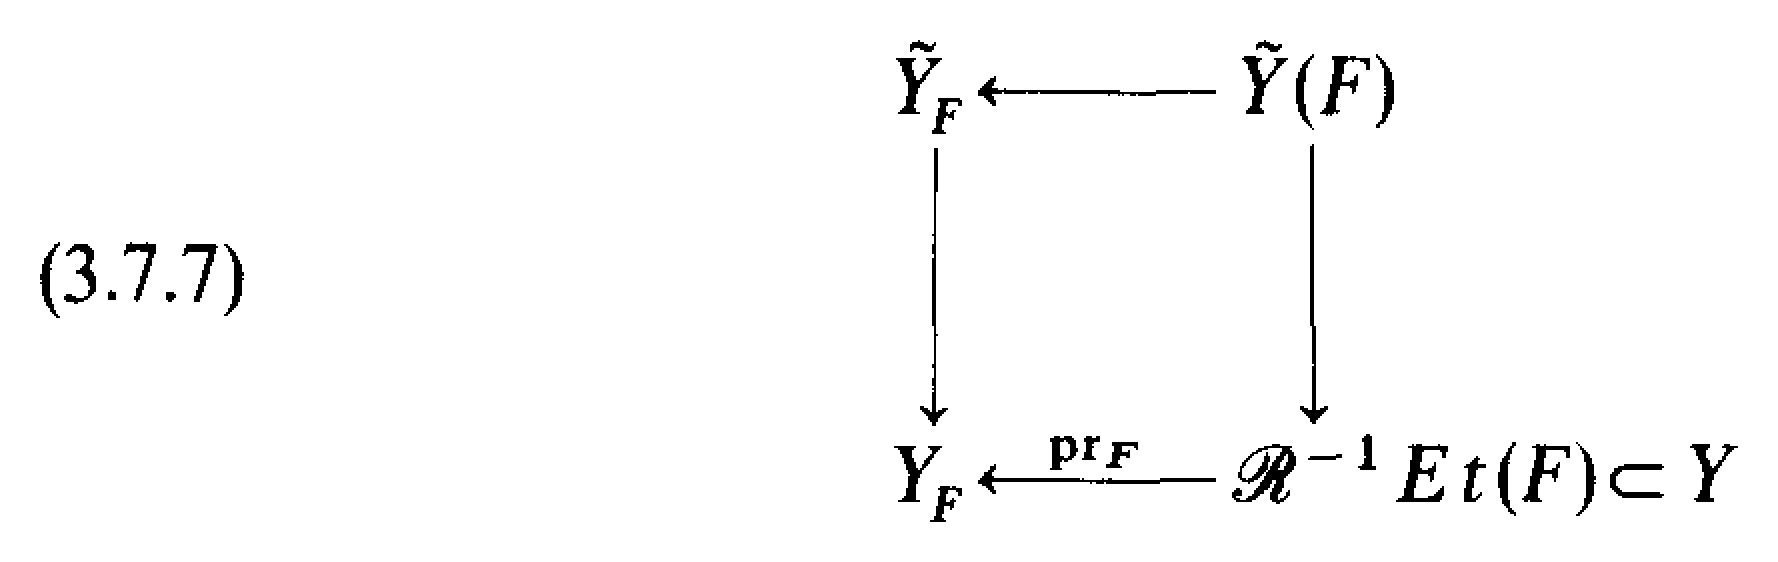
\includegraphics[width=0.80\linewidth]{P0024-A01.png}
\label{fig:p0024-a01}
\end{figure}

which sends \ensuremath{\widetilde{Y}(b(\pi{}_F(B)))\cap{}p^{-1}\mathcal{R}^{-1}\operatorname{Et}(F)} into \ensuremath{\widetilde{Y}_F(b(B))} for \ensuremath{B} a chamber of \ensuremath{I_F.} The first vertical arrow therefore also the second are coverings.\par

It is easily verified that the map \ensuremath{pr_F} of (3.7.7) is a homotopy equivalence, whence\par

\paragraph{(3.7.8) Lemma.} \ensuremath{\widetilde{Y}_F} and \ensuremath{\widetilde{Y}(F)} have the same homotopy type.

\subsubsection*{\ensuremath{D.} End of the proof.}

We prove (3.7) by induction on \ensuremath{r=dim} \ensuremath{V.} Let \ensuremath{\mathcal{U}} be the open covering of \ensuremath{\widetilde{Y}} by the \ensuremath{\widetilde{Y}(s),} for s a vertex of \ensuremath{\widehat{I}.} By (3.7.4)(i), \ensuremath{\widehat{I}} is the nerve of \ensuremath{\mathcal{U}.} By (3.7.4), (3.7.8), and the induction hypothesis, the nonempty intersections of open sets belonging to \ensuremath{\mathcal{U}} are contractible. This implies [6] that \ensuremath{\widetilde{Y}} and \ensuremath{\widehat{I}=\operatorname{Nerf}(\mathcal{U})} have the same homotopy type. The conclusion follows from (2.15).\par

\section*{4. Braid groups}

\paragraph{(4.1)} Let \ensuremath{V} be a finite-dimensional real vector space and \ensuremath{W\subset{}\operatorname{GL}(V)} a finite group generated by reflections. Assume that \ensuremath{V^W=\{0\}.} Let \ensuremath{\Phi{}} be any Euclidean structure on \ensuremath{V} invariant under \ensuremath{W,} and let \ensuremath{\mathcal{M}} be the set of hyperplanes \ensuremath{M} such that the orthogonal reflection with respect to \ensuremath{\mathcal{M}} belongs to \ensuremath{W.} One knows that

\hangindent=1.5em\noindent a) \ensuremath{(V,} \ensuremath{\mathcal{M})} satisfies 1.6 ([1] \ensuremath{V} 3.9 prop. 7);\par

\hangindent=1.5em\noindent b) \ensuremath{W} permutes the chambers of \ensuremath{(V,} \ensuremath{\mathcal{M})} in a strictly simply transitive manner ([1] \ensuremath{V} 3.2 Th. 1);\par

\hangindent=1.5em\noindent c) if \ensuremath{x\in{}V} belongs to the closed chamber \ensuremath{\overline{A},} its stabilizer is generated by the reflections in the walls of A containing \ensuremath{x} ([1] \ensuremath{V} 3.3 prop. 1);\par

\hangindent=1.5em\noindent d) (follows from c)) the group $W$ acts freely on
\[Y_W=V_C-\bigcup_{M\in\mathcal{M}}M_C.\]

By b), if \ensuremath{C_0} and \ensuremath{C_1} are two chambers, there is a unique \ensuremath{w\in{}W} such that \ensuremath{wC_0=C_1;} these \ensuremath{w} induce a transitive system of bijections between the walls of the different chambers. Passing to the quotient, one obtains a set \ensuremath{D} with dim(V) elements and, for each chamber \ensuremath{C,} a bijec-\par

% END ACCEPTED RECORD P0024

% BEGIN ACCEPTED RECORD P0025 / PRINTED 297
% source_sha256=1905043232E1DADD97696372252BB5F91C202EA1B72379E77A9FECBFE9EED4BC
% ndjson_line_sha256=5f024960ce514565263f08deea789bfdc8fe78e11b98474dcc3cd7baf1b5ba03
tion \ensuremath{\varphi{}_C} from \ensuremath{D} onto the set of walls of \ensuremath{C.} One has\par

\paragraph{(4.1.1)} \ensuremath{\varphi{}_{wC}(i)=w\varphi{}_C(i)} \ensuremath{(w\in{}W).}

For the definition of the Coxeter matrix \ensuremath{(m_{ij})_{i,j\in{}D}} and that of the Coxeter graph, we refer to [1] \ensuremath{V} 3.4.\par

\paragraph{(4.2)} Choose a chamber \ensuremath{A_0} of \ensuremath{(V,} \ensuremath{\mathcal{M}).} For \ensuremath{i\in{}D,} let \ensuremath{w_i} be the reflection in the wall \ensuremath{\varphi{}_{A_0}(i).} [1] \ensuremath{V} 3.2 Th. 1 says that \ensuremath{W} is generated by the \ensuremath{w_i,} these generators being subject only to the relations

\ensuremath{(w_iw_j)^{m_{ij}}=e.}\par

\paragraph{(4.3)} Let \ensuremath{X_W=Y_W/W:} by (4.1)d), \ensuremath{Y_W} is a covering of \ensuremath{X_W,} with group \ensuremath{W.} Let \ensuremath{y_0\in{}A_0} have image \ensuremath{x_0\in{}X_W.} For each \ensuremath{i\in{}D,} let \ensuremath{\ell{}_i'} be the homotopy class of paths in \ensuremath{Y_W,} from \ensuremath{y_0} to \ensuremath{w_i(y_0),} which, for \ensuremath{y\in{}A_0,} contains the broken line with successive vertices \ensuremath{y_0,} \ensuremath{y_0+iy_0,} \ensuremath{w_i(y_0)+iy_0,} \ensuremath{w_i(y_0).} The image \ensuremath{\ell{}_i} of \ensuremath{\ell{}_i'} in \ensuremath{X_W} is a loop based at \ensuremath{x_0.}

\paragraph{(4.4) Theorem.} (i) The fundamental group \ensuremath{\pi{}_1(X_W,} \ensuremath{x_0)} is generated by the \ensuremath{\ell{}_i;} these are subject only to the relations

\paragraph{(4.4.1)} \ensuremath{\operatorname{prod}(m_{ij};} \ensuremath{\ell{}_i,} \ensuremath{\ell{}_j)=\operatorname{prod}(m_{ji};} \ensuremath{\ell{}_j,} \ensuremath{\ell{}_i).}

\hangindent=1.5em\noindent (ii) The universal covering of \ensuremath{X_W} is contractible: \ensuremath{X_W} is a \ensuremath{K(\pi{};} 1).\par

Assertion (i) is proved in Brieskorn [3]. Another proof will be sketched in (4.18) below. As explained in the introduction, (ii) follows from (3.7) and (4.1).\par

\paragraph{(4.5)} In \S{} 1, we have drawn heavily on Garside's study [4] of Artin's braid group; from the results obtained we can now derive information about all groups of the type \ensuremath{\pi{}_1(X_W,} \ensuremath{x_0)} (Garside had already considered some of them). The translation rests on (4.6), (4.7) below.

\paragraph{(4.6)} Let \ensuremath{G=(C_0,} \ldots{}, \ensuremath{C_n)} be a gallery and \ensuremath{M_i} the wall separating \ensuremath{C_{i-1}} from \ensuremath{C_i} \ensuremath{(1\le{}i\le{}n).} One has \ensuremath{\varphi{}_{C_{i-1}}^{-1}(M_i)=\varphi{}_{C_i}^{-1}(M_i).} Let \ensuremath{\ell{}(G)} be the element \ensuremath{\varphi{}_{C_1}^{-1}(M_1)\ldots{}\varphi{}_{C_n}^{-1}(M_n)} of \ensuremath{L^{+}(D)} (0.1).

The map \ensuremath{\ell{}} induces a bijection from the set of galleries \ensuremath{G} with a given source to \ensuremath{L^{+}(D).} One has\par

\paragraph{(4.6.1)} \ensuremath{\ell{}(w(G))=\ell{}(G)} (for \ensuremath{w\in{}W);}

\paragraph{(4.6.2)} \ensuremath{\ell{}(G_0G_1)=\ell{}(G_0)\ell{}(G_1)} (for composable \ensuremath{G_0} and \ensuremath{G_1).}

Let \ensuremath{w:} \ensuremath{L(D)\longrightarrow{}W} be the homomorphism extending the map \ensuremath{i\longmapsto{}w_i} from \ensuremath{D} to \ensuremath{W.}\par

% END ACCEPTED RECORD P0025

% BEGIN ACCEPTED RECORD P0026 / PRINTED 298
% source_sha256=1905043232E1DADD97696372252BB5F91C202EA1B72379E77A9FECBFE9EED4BC
% ndjson_line_sha256=63f1baaaa4bd637dbe609c1d9681089a50fa7757b806b1810c1a9b2b092b2b51
\paragraph{(4.7) Proposition.} For every gallery \ensuremath{G} with source \ensuremath{A_0,} one has

\ensuremath{A_0.G=w(\ell{}(G))(A_0).}\par

This is an avatar of the identity\par

\ensuremath{[(w_1\ldots{}w_{n-1})w_n(w_1\ldots{}w_{n-1})^{-1}]}\par

\ensuremath{\mathbin{\cdot}[(w_1\ldots{}w_{n-2})w_{n-1}(w_1\ldots{}w_{n-2})^{-1}]\ldots{}[w_1]=w_1\ldots{}w_n.}\par

\paragraph{(4.8)} From this proposition one deduces that, for \ensuremath{w\in{}W,} the integer \ensuremath{d(A_0,} \ensuremath{w(A_0))} is the least length of words in the \ensuremath{w_i} that equal \ensuremath{w;} more precisely, \ensuremath{\ell{}} induces a bijection from the set of minimal galleries from \ensuremath{A_0} to \ensuremath{wA_0} to the set of words \ensuremath{m\in{}L(D),} of minimal length, such that \ensuremath{w=w(m).}

\paragraph{(4.9) Definition.} (i) The braid monoid \ensuremath{G^{+}} of type \ensuremath{D} is the monoid with unit generated by \ensuremath{D,} the generators \ensuremath{i\in{}D} being subject only to the relations

\paragraph{(4.9.1)} \ensuremath{\operatorname{prod}(m_{ij};} i, \ensuremath{j)=\operatorname{prod}(m_{ij};} j, i).

\hangindent=1.5em\noindent (ii) The braid group \ensuremath{G} (or generalized braid group) of type \ensuremath{D} is the group generated by \ensuremath{D,} the generators being subject to (4.9.1).\par

\paragraph{(4.10)} Notice that \ensuremath{W} also admits the presentation

\paragraph{(4.10.1)} \ensuremath{\operatorname{prod}(m_{ij};} \ensuremath{w_i,} \ensuremath{w_j)=\operatorname{prod}(m_{ij};} \ensuremath{w_j,} \ensuremath{w_i),}

\paragraph{(4.10.2)} \ensuremath{w_i^{2}=e.}

so that \ensuremath{i\longmapsto{}w_i} extends to a homomorphism from \ensuremath{G} to \ensuremath{W.}\par

\paragraph{(4.11)} One checks from the definitions that two galleries \ensuremath{G_0} and \ensuremath{G_1} with the same source are equivalent if and only if \ensuremath{\ell{}(G_0)} and \ensuremath{\ell{}(G_1)} have the same image in \ensuremath{G^{+}.} Taking account of (4.9), (1.12) therefore admits the following translation ([1] IV 1.6 prop. 5).

\paragraph{(4.12) Reminder.} Let \ensuremath{w\in{}W.} The image in \ensuremath{G^{+}} of the words \ensuremath{m\in{}L(D),} of minimal length among those such that \ensuremath{w=w(m),} depends only on \ensuremath{w.}

This image will be denoted \ensuremath{r(w);} \ensuremath{r} is a section of \ensuremath{w:} \ensuremath{G^{+}\longrightarrow{}W.} By (4.7), one has \ensuremath{r(w)=\ell{}(u(A_0,} \ensuremath{wA_0)).}\par

Similarly, [1] IV 1.4 lemma 2 corresponds to (1.11).\par

\paragraph{(4.13)} The ``quotient'' category of \ensuremath{\operatorname{Gal}_+(V,} \ensuremath{\mathcal{M})} by \ensuremath{W} is defined as follows:

\hangindent=1.5em\noindent a) Its set of objects is reduced to one element: it is\par

\ensuremath{\operatorname{Ob}(\operatorname{Gal}_+(V,} \ensuremath{\mathcal{M}))/W.}\par

% END ACCEPTED RECORD P0026

% BEGIN ACCEPTED RECORD P0027 / PRINTED 299
% source_sha256=1905043232E1DADD97696372252BB5F91C202EA1B72379E77A9FECBFE9EED4BC
% ndjson_line_sha256=d8353f6e6b2218d5882636340399152d69d005f92ef9bd224c94830d3fe8590d
\hangindent=1.5em\noindent b) The monoid of its arrows is \ensuremath{\operatorname{Fl}(\operatorname{Gal}_+(V,} \ensuremath{\mathcal{M}))/W,} and passage to the quotient\par

\ensuremath{\operatorname{Gal}_+(V,} \ensuremath{\mathcal{M})\longrightarrow{}\operatorname{Gal}_+(V,} \ensuremath{\mathcal{M})/W}\par

is a functor.\par

This category, having only one object, is identified with the monoid of its arrows. By (4.6.1), (4.6.2), and (4.11), \ensuremath{\ell{}} identifies this monoid with \ensuremath{G^{+}.}\par

Similarly one defines \ensuremath{\operatorname{Gal}(V,} \ensuremath{\mathcal{M})/W.} This category has only one object and, by its universal property, \ensuremath{\ell{}} extends to an isomorphism from the group of its arrows to \ensuremath{G:}\par

\begin{figure}[htbp]
\centering
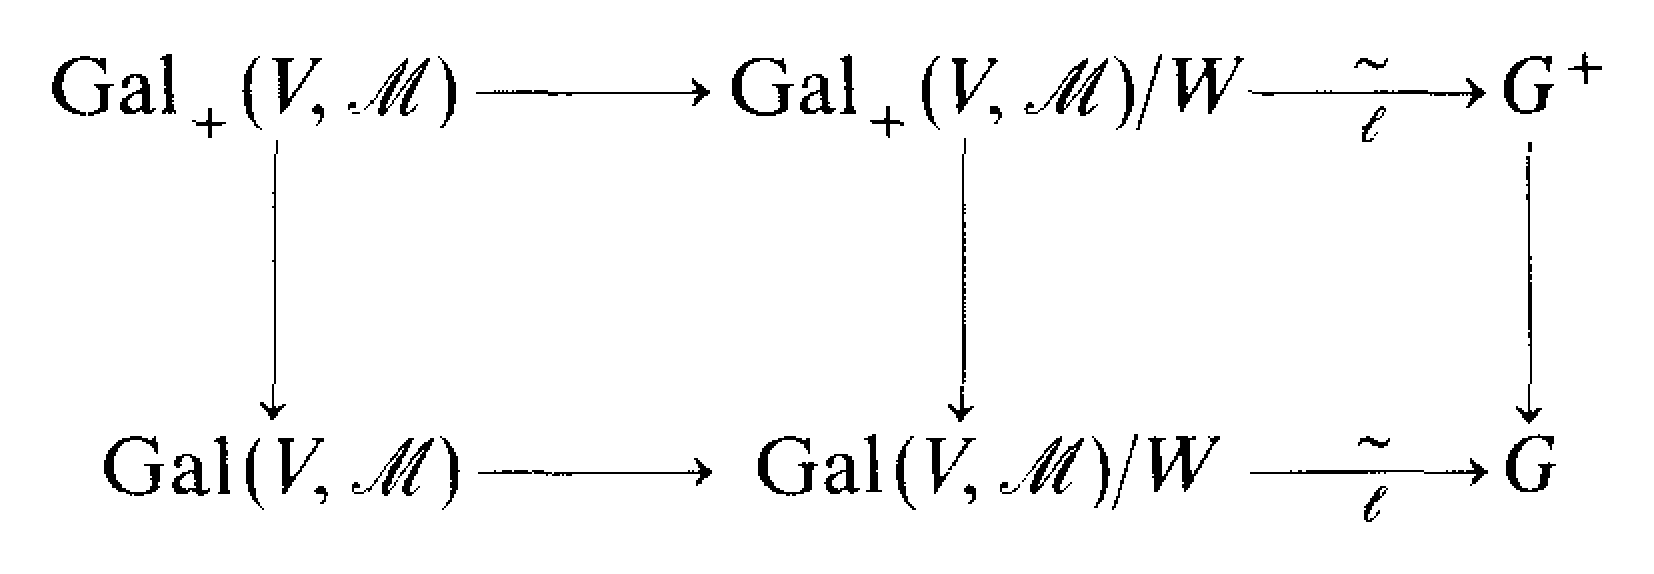
\includegraphics[width=0.78\linewidth]{P0027-A01.png}
\label{fig:p0027-a01}
\end{figure}

\paragraph{(4.14) Theorem.} (i) In \ensuremath{G^{+},} left and right translations are injective.

\hangindent=1.5em\noindent (ii) \ensuremath{G^{+}} satisfies the Öre condition on the left and on the right. It follows from (i) that \ensuremath{G^{+}} embeds in \ensuremath{G.}\par

\hangindent=1.5em\noindent (iii) For \ensuremath{J} a subset of \ensuremath{D,} let \ensuremath{G_J^{+}} (resp. \ensuremath{G_J)} be the submonoid (resp. subgroup) of \ensuremath{G^{+}} (resp. \ensuremath{G)} generated by the \ensuremath{i\in{}J.} Then the evident map identifies \ensuremath{G_J^{+}} (resp. \ensuremath{G_J)} with the braid monoid (resp. braid group) of type \ensuremath{J.}\par

\hangindent=1.5em\noindent (iv) One has \ensuremath{G_J^{+}=G_J\cap{}G^{+}.}\par

\hangindent=1.5em\noindent \ensuremath{(v)} If \ensuremath{J} and \ensuremath{K} are two subsets of \ensuremath{D,} one has \ensuremath{G_J\cap{}G_K=G_{J\cap{}K}.}\par

\hangindent=1.5em\noindent (vi) Let n(i) be the number of elements of \ensuremath{G^{+}} of length i, and put \ensuremath{f=\sum{}n(i)t^i.} For \ensuremath{J\subset{}D,} let m(J) be the number of walls passing through the intersection of the walls of an (arbitrary) chamber A, indexed by \ensuremath{J} \ensuremath{(=the} number of reflections in the Weyl group \ensuremath{W_J).} One has\par

\[
f=(\sum{}_{J\subset{}D}(-1)^{|J|}t^{m(J)})^{-1}
\]

These assertions translate respectively: (i): (1.1)(i) and (ii); (ii): (1.26)(ii) and its transform by passage to opposite galleries (cf. also (4.16) below); (iii): (1.30); (iv): (1.32); \ensuremath{(v):} (1.31); (vi): (1.21) (the \ensuremath{f_A} of loc. cit. are all equal to f).\par

Let \ensuremath{x,} \ensuremath{y\in{}G^{+}.} We say that \ensuremath{x} begins with \ensuremath{y} if there exists \ensuremath{z} in \ensuremath{G^{+}} with \ensuremath{x=yz.} Proposition (1.19)(iii) translates as follows\par

\paragraph{(4.15) Lemma.} Let \ensuremath{x\in{}G^{+}.} There exists a chamber \ensuremath{C} such that, for every \ensuremath{w\in{}W,} \ensuremath{x} begins with \ensuremath{r(w)} if and only if \ensuremath{wA_0\in{}D(A_0,} \ensuremath{C).}

% END ACCEPTED RECORD P0027

% BEGIN ACCEPTED RECORD P0028 / PRINTED 300
% source_sha256=1905043232E1DADD97696372252BB5F91C202EA1B72379E77A9FECBFE9EED4BC
% ndjson_line_sha256=2b92ee436d427e9e6f1e23d4b4dc11dd06a5149e2832d5b1e499006346ad9923
\paragraph{(4.16)} Let \ensuremath{J} be a subset of \ensuremath{D} and \ensuremath{P} the intersection of the walls \ensuremath{\varphi{}_{A_0}(i)} \ensuremath{(i\in{}J).} Let \ensuremath{\Delta{}(J)} be the element \ensuremath{\ell{}(u(A_0,} \ensuremath{A_0.\Delta{}(P)))} of \ensuremath{G^{+};} put \ensuremath{\Delta{}=\Delta{}(D).} Let \ensuremath{i\longmapsto{}\bar{\imath}=\varphi{}_{-C}^{-1}\varphi{}_C(i)} be the opposition involution of \ensuremath{D.} We also denote by \ensuremath{w\longmapsto{}\overline{w}} the automorphisms of \ensuremath{L^{+}(D),} \ensuremath{G^{+},} and \ensuremath{G} that send i to \ensuremath{\bar{\imath}} (one has \ensuremath{m_{ij}=m_{\overline{i}\overline{j}}).} Translating (1.26) with the aid of (4.4), one finds that for \ensuremath{g} in \ensuremath{G^{+}} or \ensuremath{G,}

\paragraph{(4.16.1)} \ensuremath{g\Delta{}=\Delta{}\overline{g}.}

In particular, \ensuremath{\Delta{}^{2}} is central.\par

For every \ensuremath{i\in{}D,} \ensuremath{\Delta{}} ``begins'' with i: one has \ensuremath{\Delta{}=ix,} in \ensuremath{G^{+}.} Hence\par

\paragraph{(4.17) Proposition.} \ensuremath{G} is obtained from \ensuremath{G^{+}} by making the central element \ensuremath{\Delta{}^{2}} invertible.

\paragraph{(4.18)} The description (2.11), \ensuremath{(2.5)-(2.7)} of the building I attached to \ensuremath{(V,} \ensuremath{\mathcal{M})} can be translated as follows.

\hangindent=1.5em\noindent a) The set of vertices of I is\par

\[
I^{0}=\coprod_{i\in{}D} G/G_{D-{i}}
\]

\hangindent=1.5em\noindent b) For a set of vertices to span a simplex, it is necessary and sufficient that it be contained in the set of classes \ensuremath{gG_{D-{i}},} for some \ensuremath{g\in{}G.}\par

\hangindent=1.5em\noindent c) The fundamental sphere \ensuremath{S_0=S(A_0)} is the union of the fundamental simplex, spanned by the lateral classes of \ensuremath{e} in the \ensuremath{G/G_{D-{i}},} and of its transforms by the \ensuremath{r(w)} \ensuremath{(w\in{}W).}\par

The preceding description makes evident a left action of \ensuremath{G} on I. It respects the set of spheres \ensuremath{S(A)} and the correspondence \ensuremath{A\longmapsto{}S(A).}\par

By transport of structure, \ensuremath{G} acts on the covering \ensuremath{\widetilde{Y}_W} of \ensuremath{Y_W} (3.6), and one has an equivariant morphism\par

\ensuremath{(G-\widetilde{Y}_W)\longrightarrow{}(W-Y_W).}\par

It follows that \ensuremath{G} is the fundamental group of \ensuremath{X_W=Y_W/W,} and (4.4)(i).\par

\paragraph{(4.19)} For completeness, let us show that the word problem, the conjugacy problem, and the question of computing the center of \ensuremath{G} can be solved as in [4]. If the Coxeter graph \ensuremath{D} of \ensuremath{W} is a disjoint union of graphs \ensuremath{D_\alpha{},} the braid group of type \ensuremath{D} is the product of the braid groups of types \ensuremath{D_\alpha{}.} The essential case is therefore that of a connected graph \ensuremath{D.}

\paragraph{(4.20)} The word problem: there is a decision procedure for determining whether two elements \ensuremath{m} and \ensuremath{n} of L(D) have the same image in \ensuremath{G.}

% END ACCEPTED RECORD P0028

% BEGIN ACCEPTED RECORD P0029 / PRINTED 301
% source_sha256=1905043232E1DADD97696372252BB5F91C202EA1B72379E77A9FECBFE9EED4BC
% ndjson_line_sha256=7cd8fb58cbb091216c59362af8a35f34063f8d5cf397e11af49da3600c0a8d98
\hangindent=1.5em\noindent a) Whether \ensuremath{m} and \ensuremath{n} in \ensuremath{L^{+}(D)} have the same image in \ensuremath{G^{+}} is decidable, because the imposed relations do not change the length of the words, and there are only finitely many words of a given length. One may also use (1.22).\par

\hangindent=1.5em\noindent b) For any \ensuremath{m_i} \ensuremath{(i=1,} 2) in the free group L(D) generated by \ensuremath{D,} one can compute \ensuremath{m_i'\in{}L^{+}(D)} and \ensuremath{k\ge{}0} such that \ensuremath{m_i} and \ensuremath{m_i'\Delta{}^{-k}} have the same image in \ensuremath{G} (cf. (4.17)); \ensuremath{m_1} and \ensuremath{m_2} then have the same image in \ensuremath{G} if and only if \ensuremath{m_1'} and \ensuremath{m_2'} have the same image in \ensuremath{G^{+}.}\par

\paragraph{(4.21) Theorem.} If the Coxeter graph \ensuremath{D} is connected (nonempty) and the opposition involution is trivial (resp. nontrivial), the center of \ensuremath{G} is infinite monogenic, generated by \ensuremath{\Delta{}} (resp. \ensuremath{\Delta{}^{2}).}

Consider the following property of \ensuremath{x\in{}G^{+}.}\par

(*) For every \ensuremath{i\in{}D,} there exists \ensuremath{i'\in{}D} such that \ensuremath{ix=xi'.}\par

It is enough to prove that, if \ensuremath{x} satisfies (*) and \ensuremath{x\ne{}e,} then \ensuremath{x=\Delta{}y} with \ensuremath{y\in{}G^{+}.} By induction on the length of \ensuremath{x,} it will follow that if \ensuremath{x} satisfies (*), \ensuremath{x} is of the form \ensuremath{\Delta{}^k.} In particular, the center of \ensuremath{G^{+}} is contained in the set of the \ensuremath{\Delta{}^k} \ensuremath{(k\ge{}0);} by (4.14)(i) and (4.17), the center of \ensuremath{G} is contained in the set of the \ensuremath{\Delta{}^k} \ensuremath{(k\in{}\mathbb{Z}),} and the assertion follows from (4.16.1).\par

Let \ensuremath{x\in{}G^{+}} satisfy (*). Let \ensuremath{C} be as in (4.15), and let \ensuremath{w} be the image in \ensuremath{W} of \ensuremath{\ell{}u(A_0,} \ensuremath{C).} We may write \ensuremath{x=r(w)y,} with \ensuremath{y\in{}G^{+}.} Let \ensuremath{i\in{}D.} By (*), \ensuremath{ix=r(w)yi'} begins with \ensuremath{r(w);} by (1.23), it follows that ir(w) begins with \ensuremath{r(w):} \ensuremath{ir(w)=r(w)i''.} In particular, for every i, there exists \ensuremath{i''} with \ensuremath{iw=wi'';} this means that every wall of \ensuremath{A_0} is also a wall of \ensuremath{wA_0.} Among the \ensuremath{2^{|D|}} open simplicial cones bounded by the walls of \ensuremath{A_0,} only \ensuremath{A_0} and \ensuremath{-A_0} are chambers: they are the only ones whose angles between the faces are all \ensuremath{\le{}\pi{}/2} (the connectedness of \ensuremath{D} is used here). If \ensuremath{x\ne{}e,} then \ensuremath{w\ne{}e} and hence \ensuremath{wA_0=-A_0.} Since then \ensuremath{\Delta{}=r(w),} this completes the proof.\par

\paragraph{(4.22)} The derived group. Let \ensuremath{D'} be the graph having \ensuremath{D} as its set of vertices, two vertices being joined by an edge if and only if \ensuremath{m_{ij}} is odd. Let \ensuremath{D_0} be the set of connected components of \ensuremath{D'.} Define an epimorphism

Lg: \ensuremath{G\longrightarrow{}\mathbb{Z}^{D_0}}\par

by sending i to the basis vector indexed by the connected component of i in \ensuremath{D'.} One verifies at once that Lg identifies \ensuremath{\mathbb{Z}^{D_0}} with the largest abelian quotient of \ensuremath{G.}\par

\paragraph{(4.23)} The conjugacy problem. The problem is to give a decision procedure for determining whether two elements \ensuremath{x} and \ensuremath{y} of \ensuremath{G} (given explicitly as images of words in L(D)) are conjugate. Since \ensuremath{\Delta{}^{2}} is central, \ensuremath{\Delta{}^{-2k}a} and \ensuremath{\Delta{}^{-2k}b} are conjugate if and only if a and b are. By

% END ACCEPTED RECORD P0029

% BEGIN ACCEPTED RECORD P0030 / PRINTED 302
% source_sha256=1905043232E1DADD97696372252BB5F91C202EA1B72379E77A9FECBFE9EED4BC
% ndjson_line_sha256=a2b2b75d158618547f1ba812fd4fa1304fa18dc8fcfa5e6df273345123e859e4
(4.17), it therefore suffices to treat the case where \ensuremath{x,} \ensuremath{y\in{}G^{+}.} Similarly, if \ensuremath{x} and \ensuremath{y} are conjugate, there exists a in \ensuremath{G^{+}} such that \ensuremath{xa=ay.} If \ensuremath{x} and \ensuremath{y} are conjugate, \ensuremath{\operatorname{Lg}(x)=\operatorname{Lg}(y).} There are only finitely many \ensuremath{x\in{}G^{+}} of given ``length'' \ensuremath{\operatorname{Lg}(x),} and \ensuremath{W} is finite. The existence of a decision procedure then follows from (4.20) and the following lemma.\par

\paragraph{(4.24) Lemma.} Let \ensuremath{x,} \ensuremath{y} be in \ensuremath{G^{+}.} If \ensuremath{x} and \ensuremath{y} are conjugate, there exists a sequence \ensuremath{x_0=x,} \ensuremath{x_1,} \ldots{}, \ensuremath{x_n=y} of elements of \ensuremath{G^{+}} and a sequence of elements \ensuremath{w_i} of \ensuremath{W} such that

\ensuremath{x_{i+1}r(w_i)=r(w_i)x_i.}\par

Let \ensuremath{a\in{}G^{+}} be such that \ensuremath{xa=ay.} Put \ensuremath{a=r(w_0)\ldots{}r(w_{n-1}),} where \ensuremath{w_i} is the element of \ensuremath{W} of maximum length such that \ensuremath{r(w_i)\ldots{}r(w_{n-1})} can be written in the form \ensuremath{r(w_i)b_i} with \ensuremath{b_i\in{}G^{+}} (4.15). Let \ensuremath{a_i=r(w_0)\ldots{}r(w_i).} We shall prove that \ensuremath{x_i=a_i^{-1}xa_i} lies in \ensuremath{G^{+},} so that the \ensuremath{x_i} and \ensuremath{w_i} answer the problem.\par

It follows from (1.23) that, for every \ensuremath{w\in{}W,} if xa begins with \ensuremath{r(w),} then \ensuremath{xr(w_0)} also begins with \ensuremath{r(w).} In particular, since \ensuremath{xa=ay=r(w_0)b_0y} begins with \ensuremath{r(w_0),} \ensuremath{xr(w_0)=r(w_0)x_1} with \ensuremath{x_1\in{}G^{+}.} The proof is completed by induction on \ensuremath{n.}\par

\paragraph{Remark.} Let \ensuremath{\sigma{}} be an automorphism of the Coxeter graph \ensuremath{D,} and again denote by \ensuremath{\sigma{}} the corresponding automorphism of \ensuremath{G.} One has \ensuremath{\Delta{}^\sigma{}=\Delta{}.} The preceding arguments still apply to the question of deciding, for \ensuremath{x,} \ensuremath{y\in{}G,} whether there exists a in \ensuremath{G} such that \ensuremath{xa=a^\sigma{}y.} We reduce to taking \ensuremath{x,} \ensuremath{y,} and a in \ensuremath{G^{+}.} In that case and, with the preceding notation, if \ensuremath{xa=a^\sigma{}y,} the \ensuremath{(a_i^{-1})^\sigma{}xa_i} lie in \ensuremath{G^{+}.} Taking for \ensuremath{\sigma{}} the involution \ensuremath{i\longmapsto{}\bar{\imath},} one obtains a criterion analogous to (4.24) for the conjugacy of \ensuremath{\Delta{}x} and \ensuremath{\Delta{}y} \ensuremath{(x,} \ensuremath{y\in{}G^{+}).}

\section*{Bibliography}\begingroup\small

The reader will find a more complete bibliography on braid groups in [2].\par

\noindent 1. Bourbaki, \ensuremath{N.:} Groupes et algèbres de Lie. Chap. 4, 5, 6. Paris: Hermann 1968.\par

\noindent 2. Brieskorn, \ensuremath{E.:} Sur les groupes de tresses. Sém. Bourbaki 401, nov. 71.\par

\noindent 3. Brieskorn, \ensuremath{E.:} Die Fundamentalgruppe des Raumes der regulären Orbits einer endlichen komplexen Spiegelungsgruppe. Inventiones math. 12, \ensuremath{57-61} (1971).\par

\noindent 4. Garside, \ensuremath{F.} A.: The braid groups and other groups. Quat. \ensuremath{J.} Math. Oxford, 2nd ser. 20, \ensuremath{235-254} (1969).\par

\noindent 5. Tits, \ensuremath{J.:} Normalisateurs de Tores. I Groupes de Coxeter étendus. \ensuremath{J.} of algebra 4 (1), \ensuremath{96-116} (1966).\par

\noindent 6. Weil, A.: Sur les théorèmes de De Rham. Comm. Math. Helv. 26 (1952).\par

\begin{flushleft}
Pierre Deligne\\
Institut des Hautes Études Scientifiques\\
35 Route de Chartres\\
F-91440 Bures-sur-Yvette\\
France
\end{flushleft}

(Received 24 April 1972)\par

% END ACCEPTED RECORD P0030

\endgroup
\end{document}
